\documentclass[11pt, oneside]{book}

% ============================================================
%  Advanced Scheduling Systems — shared preamble
% ============================================================

\usepackage[a4paper,
            top=25mm, bottom=25mm,
            left=25mm, right=55mm,   % wide right margin for notes
            marginparwidth=45mm,
            marginparsep=4mm]{geometry}

% --- typography & encoding ---
\usepackage[T1]{fontenc}
\usepackage[utf8]{inputenc}
\usepackage{microtype}
\usepackage{lmodern}

% --- math ---
\usepackage{amsmath, amssymb, amsthm, mathtools}

% --- margin notes ---
\usepackage{marginnote}
\usepackage{sidenotes}          % \sidenote{}, \marginnote{}

% --- code listings ---
\usepackage{listings}
\usepackage{xcolor}

\definecolor{codebg}{RGB}{245,245,245}
\definecolor{codecomment}{RGB}{100,100,100}
\definecolor{codekw}{RGB}{0,0,200}
\definecolor{codestr}{RGB}{163,21,21}

\lstset{
  backgroundcolor=\color{codebg},
  basicstyle=\ttfamily\small,
  keywordstyle=\color{codekw}\bfseries,
  commentstyle=\color{codecomment}\itshape,
  stringstyle=\color{codestr},
  numbers=left, numberstyle=\tiny\color{gray},
  numbersep=6pt,
  breaklines=true,
  frame=single, framesep=4pt,
  captionpos=b,
  tabsize=4,
  showstringspaces=false,
}

% --- pseudocode ---
\usepackage[ruled, vlined, linesnumbered]{algorithm2e}
\SetAlgoLined
\DontPrintSemicolon

% --- graphics / figures ---
\usepackage{float}      % provides [H] float placement
\usepackage{graphicx}
\usepackage{caption}    % provides \caption*{} for unnumbered captions
\usepackage{tikz}
\usetikzlibrary{arrows.meta, positioning, shapes.geometric, decorations.pathmorphing, decorations.pathreplacing}

% --- hyperlinks ---
\usepackage[colorlinks=true, linkcolor=blue!70!black,
            citecolor=green!50!black, urlcolor=blue]{hyperref}

% --- misc ---
\raggedbottom
\usepackage{enumitem}
\usepackage{booktabs}
\usepackage{cleveref}

% --- intermezzo box ---
\usepackage[framemethod=tikz]{mdframed}
\newmdenv[
  skipabove=\bigskipamount,
  skipbelow=\bigskipamount,
  backgroundcolor=orange!4,
  hidealllines=true,
  innertopmargin=12pt,
  innerbottommargin=12pt,
  innerleftmargin=14pt,
  innerrightmargin=12pt,
]{intermezzoframe}
\newenvironment{intermezzo}[1]{%
  \begin{adjustwidth}{-5mm}{-35mm}%
  \begin{intermezzoframe}%
  \noindent{\small\sffamily\bfseries\color{orange!60!black}%
    \raisebox{0.5pt}{\rule{6pt}{6pt}}\enspace%
    Intermezzo\enspace---\enspace#1}%
  \par\vspace{6pt}%
}{%
  \end{intermezzoframe}%
  \end{adjustwidth}%
}

% --- formal-details box ---
\usepackage{changepage}
\newmdenv[
  skipabove=\bigskipamount,
  skipbelow=\bigskipamount,
  backgroundcolor=teal!4,
  hidealllines=true,
  innertopmargin=12pt,
  innerbottommargin=12pt,
  innerleftmargin=14pt,
  innerrightmargin=12pt,
]{formaldetailsframe}
\newenvironment{formaldetails}[1][]{%
  \begin{adjustwidth}{-5mm}{-35mm}%
  \begin{formaldetailsframe}%
  \noindent{\small\sffamily\bfseries\color{teal!60!black}%
    \raisebox{0.5pt}{\rule{6pt}{6pt}}\enspace%
    Formal details%
    \if\relax\detokenize{#1}\relax\else
      \enspace---\enspace#1%
    \fi}%
  \par\vspace{6pt}%
}{%
  \end{formaldetailsframe}%
  \end{adjustwidth}%
}

% --- loop-invariant proof structure ---
\newlist{loopproof}{description}{1}
\setlist[loopproof]{
  font=\normalfont\small\itshape,
  leftmargin=3.2cm,
  labelwidth=3.0cm,
  labelsep=0.2cm,
  style=sameline,
  topsep=3pt,
  itemsep=4pt,
  parsep=0pt,
}
\newcommand{\lprulesep}{%
  \vspace{4pt}{\color{blue!20}\hrule height 0.4pt}\vspace{6pt}%
}

% ---- theorem environments ----
\theoremstyle{plain}
\newtheorem{theorem}{Theorem}[section]
\newtheorem{lemma}[theorem]{Lemma}
\newtheorem{corollary}[theorem]{Corollary}
\newtheorem{proposition}[theorem]{Proposition}

\theoremstyle{definition}
\newtheorem{definition}[theorem]{Definition}
\newtheorem{example}[theorem]{Example}
\newtheorem{problem}[theorem]{Problem}

\theoremstyle{remark}
\newtheorem{remark}[theorem]{Remark}
\newtheorem{note}[theorem]{Note}
\newtheorem{observation}[theorem]{Observation}
\newtheorem{exercise}[theorem]{Exercise}

% ---- theorem environment styles (colored left bar) ----
\mdfdefinestyle{thmbar}{%
  skipabove=7pt, skipbelow=5pt,
  topline=false, rightline=false, bottomline=false, leftline=true,
  linewidth=2.5pt,
  innerleftmargin=9pt, innerrightmargin=4pt,
  innertopmargin=3pt,  innerbottommargin=3pt,
}
\surroundwithmdframed[style=thmbar,
  linecolor=blue!60!black, backgroundcolor=blue!4]{theorem}
\surroundwithmdframed[style=thmbar,
  linecolor=blue!60!black, backgroundcolor=blue!4]{lemma}
\surroundwithmdframed[style=thmbar,
  linecolor=blue!60!black, backgroundcolor=blue!4]{corollary}
\surroundwithmdframed[style=thmbar,
  linecolor=blue!60!black, backgroundcolor=blue!4]{proposition}
\surroundwithmdframed[style=thmbar,
  linecolor=teal!65!black,  backgroundcolor=teal!4]{definition}
\surroundwithmdframed[style=thmbar,
  linecolor=orange!70!black, backgroundcolor=orange!5]{example}
\surroundwithmdframed[style=thmbar,
  linecolor=violet!60!black, backgroundcolor=violet!4]{exercise}
\surroundwithmdframed[style=thmbar,
  linecolor=violet!60!black, backgroundcolor=violet!4]{problem}
\surroundwithmdframed[style=thmbar,
  linecolor=gray!50, backgroundcolor=gray!4]{remark}
\surroundwithmdframed[style=thmbar,
  linecolor=gray!50, backgroundcolor=gray!4]{note}
\surroundwithmdframed[style=thmbar,
  linecolor=gray!50, backgroundcolor=gray!4]{observation}

% ---- custom margin-note shorthand ----
\newcommand{\aside}[2][0pt]{%
  \marginnote{\footnotesize\itshape #2}[#1]%
}

% ---- scheduling notation ----
\newcommand{\Cmax}{C_{\max}}                     % makespan
\newcommand{\Lmax}{L_{\max}}                     % maximum lateness
\newcommand{\wC}{\sum w_j C_j}                   % weighted completion time
\newcommand{\wT}{\sum w_j T_j}                   % weighted tardiness

% ---- complexity shortcuts ----
\newcommand{\Oh}[1]{\mathcal{O}\!\left(#1\right)}
\newcommand{\Th}[1]{\Theta\!\left(#1\right)}
\newcommand{\Om}[1]{\Omega\!\left(#1\right)}
\newcommand{\NP}{\mathsf{NP}}


% ============================================================
\title{\textbf{Advanced Scheduling Systems}\\[4pt]
       \large Lecture Notes}
\author{Luca Simonetti}
\date{2025--2026}
% ============================================================

\begin{document}

\maketitle
\tableofcontents

% ================================================================
\chapter{Introduction to Scheduling}
% ================================================================
% ============================================================
%  Lecture 1 — Course overview & Project Scheduling
% ============================================================

\section{Course Overview}
\label{sec:course-overview}

This course studies \emph{discrete optimisation problems}%
\aside{Discrete = integer-valued decisions: pick item 1, 2, 3\ldots{}
not a continuous value like 0.37.}
and, crucially, how to \emph{implement} algorithms that solve them.
Think of it as \emph{applied operations research}: we take the
mathematical models you have seen in Operations Research and turn
them into running code.

\medskip\noindent
The programme breaks into four blocks:

\begin{enumerate}[leftmargin=2em]
  \item \textbf{Problem survey} (Lectures 1--4).
    A tour of scheduling, timetabling, and logistics problems,
    together with the first solving technique: greedy algorithms.
  \item \textbf{Constraint modelling with MiniZinc.}
    We write a mathematical specification of the problem in the
    MiniZinc language; an underlying constraint-programming
    solver does the rest.
  \item \textbf{Advanced C++ and frameworks.}
    Inheritance, virtual functions, abstract classes, and the
    object-oriented framework we use for local search.
  \item \textbf{Solving techniques} (implemented in C++).
    Greedy, enumeration/backtracking, constraint programming
    (via MiniZinc), local search, and metaheuristics.
    Each technique is studied briefly in theory, then immediately
    applied to a concrete problem.
\end{enumerate}

\begin{remark}
  The exam is a \textbf{project}: choose a problem (proposed by
  the instructor or negotiated), solve it with at least two
  different techniques, and compare the results.
  Groups of at most two people; individual contributions
  are assessed during an oral discussion.
\end{remark}


% ============================================================
\section{Project Scheduling}
\label{sec:project-scheduling}
% ============================================================

Every project---building a house, developing a product, installing
a software stack---consists of activities with dependencies between
them.\aside{\texttt{apt install} internally solves
a project-scheduling instance over
package dependencies.}
The \emph{project scheduling problem} asks: given the activities
and their dependencies, when should each activity start so that the
whole project finishes as early as possible?

% ------------------------------------------------------------
\subsection{Problem definition}
\label{ssec:ps-definition}
% ------------------------------------------------------------

\begin{definition}[Project Scheduling Problem]
\label{def:project-scheduling}
We are given:
\begin{itemize}[nosep]
  \item a set of $n$ \emph{jobs} (activities) $\{1,\dots,n\}$,
        each with integer duration $d_i$;
  \item a set of \emph{precedence constraints}
        $P \subseteq \{1,\dots,n\}^2$,
        forming a \textbf{DAG} (directed acyclic graph):
        $(i,j)\in P$ means job~$j$ cannot start before job~$i$
        finishes.
\end{itemize}
We must assign a \emph{start time} $S_i\ge 0$ to every job
so that:
\begin{enumerate}[nosep]
  \item all precedences are respected:
        $S_j \ge S_i + d_i$ for every $(i,j)\in P$;
  \item the \emph{makespan} $\Cmax = \max_{i} (S_i + d_i)$
        is minimised.
\end{enumerate}
The completion time of job~$i$ is $C_i = S_i + d_i$.
\end{definition}

Let's unpack this.  We have a collection of jobs, each taking a
known amount of time.  Some jobs depend on others: job~$j$ can
only begin once every predecessor has finished.  The dependencies
form a directed acyclic graph---a DAG---because a cycle would make
the problem infeasible (if $A$ must precede~$B$ and $B$ must
precede~$A$, nothing can ever start).
Our goal is a single number: the makespan $\Cmax$, i.e.\ the
moment the \emph{last} job finishes.  We want it as small as
possible.

\begin{example}[Seven-job instance]
\label{ex:seven-jobs}
Consider seven jobs with the following durations and precedence
graph:

\begin{figure}[H]
\centering
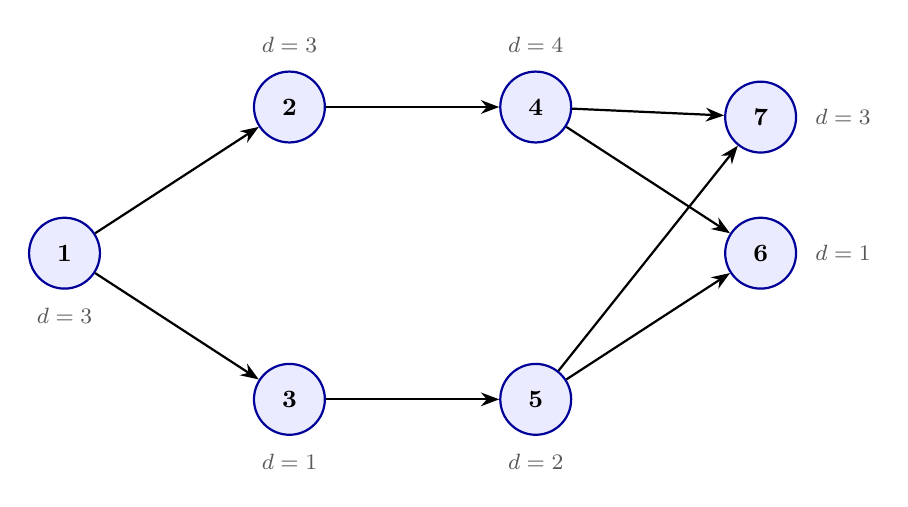
\begin{tikzpicture}[
    job/.style={circle, draw=blue!60!black, fill=blue!8,
                minimum size=9mm, font=\small\bfseries},
    dur/.style={font=\footnotesize, text=gray!70!black},
    ->, >=Stealth, thick, node distance=18mm and 22mm
  ]
  % nodes
  \node[job] (1) {1};
  \node[job, above right=12mm and 22mm of 1] (2) {2};
  \node[job, below right=12mm and 22mm of 1] (3) {3};
  \node[job, right=22mm of 2] (4) {4};
  \node[job, right=22mm of 3] (5) {5};
  \node[job, above right=12mm and 22mm of 5] (6) {6};
  \node[job, above=8mm of 6] (7) {7};

  % durations (below each node)
  \node[dur, below=1mm of 1] {$d=3$};
  \node[dur, above=1mm of 2] {$d=3$};
  \node[dur, below=1mm of 3] {$d=1$};
  \node[dur, above=1mm of 4] {$d=4$};
  \node[dur, below=1mm of 5] {$d=2$};
  \node[dur, right=1mm of 6] {$d=1$};
  \node[dur, right=1mm of 7] {$d=3$};

  % arcs
  \draw (1) -- (2);
  \draw (1) -- (3);
  \draw (2) -- (4);
  \draw (3) -- (5);
  \draw (4) -- (6);
  \draw (5) -- (6);
  \draw (4) -- (7);
  \draw (5) -- (7);
\end{tikzpicture}
\caption{Precedence DAG for the seven-job instance
         (\cref{ex:seven-jobs}).
         Each node shows the job index; durations are labelled
         alongside.}
\label{fig:seven-job-dag}
\end{figure}

\noindent
Reading the graph: job~1 must finish before jobs~2 and~3 can
start; job~4 requires job~2; job~5 requires job~3; both jobs~6
and~7 require jobs~4 and~5.
\end{example}


% ------------------------------------------------------------
\subsection{What we leave out (for now)}
\label{ssec:ps-simplifications}
% ------------------------------------------------------------

The formulation above is deliberately simple.  Real-world projects
involve several complications that we set aside here but will
revisit in later lectures:

\begin{itemize}[nosep]
  \item \textbf{Resources.}
    Two independent jobs may still conflict if they both need the
    same machine or worker.
    Resource constraints turn the problem from polynomial to
    $\NP$-hard.
  \item \textbf{Release dates and deadlines.}
    A job may not be available before a certain date, or may have
    a hard deadline.
  \item \textbf{Uncertain durations.}
    In practice durations are stochastic (it might rain, a
    delivery might be late).
    One then minimises expected or worst-case makespan---this
    belongs to the Project Management course.
  \item \textbf{Generalised precedences.}
    Start-to-start, finish-to-finish, or time-lag constraints
    (e.g.\ concrete must be poured within a window after mixing).
  \item \textbf{Variable durations with costs.}
    Crashing: pay more to shorten a job.  This introduces a
    cost--time trade-off (multi-objective).
\end{itemize}


% ============================================================
\section{The Critical Path Method (CPM)}
\label{sec:cpm}
% ============================================================

The Critical Path Method is a classical greedy algorithm that
solves the basic project scheduling problem
(\cref{def:project-scheduling}) \emph{optimally}.%
\aside{Walker \& Kelley, late 1950s.
Originally for plant maintenance
shutdowns at DuPont.}

The idea is disarmingly simple: schedule every job as early as
possible, respecting precedences.  We formalise this in two
passes---forward and backward---and then combine them to identify
the \emph{critical path}.

% ------------------------------------------------------------
\subsection{CPM Forward (earliest schedule)}
\label{ssec:cpm-forward}
% ------------------------------------------------------------

\begin{definition}[CPM Forward]
\label{def:cpm-forward}
Process jobs in \emph{topological order} of the precedence DAG:
\begin{enumerate}[nosep]
  \item For every job~$i$ with no predecessors, set $S_i = 0$.
  \item For every other job~$i$ (once all predecessors are
        scheduled):
        \[
          S_i = \max_{(k,i)\in P}\; C_k
              = \max_{(k,i)\in P}\; (S_k + d_k).
        \]
  \item Set $C_i = S_i + d_i$.
\end{enumerate}
The makespan is $\Cmax = \max_{i=1}^{n} C_i$.
\end{definition}

In words: each job starts at the earliest moment all its
predecessors have finished.  We simply walk through the DAG
from sources to sinks, computing start and finish times as we go.

\begin{example}[CPM Forward on the seven-job instance]
\label{ex:cpm-forward}
Applying CPM Forward to \cref{ex:seven-jobs}:

\begin{figure}[H]
\centering
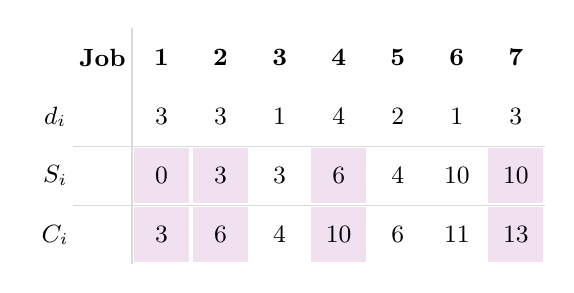
\begin{tikzpicture}[
    cell/.style={minimum width=7mm, minimum height=7mm,
                 font=\small, anchor=center},
    hdr/.style={cell, font=\small\bfseries},
    crit/.style={fill=violet!12},
    x=7.5mm, y=7.5mm
  ]
  % header row
  \foreach \j/\lbl in {1/Job, 2/1, 3/2, 4/3, 5/4, 6/5, 7/6, 8/7} {
    \node[hdr] at (\j, 4) {\lbl};
  }
  % d_i
  \node[cell, font=\small\itshape] at (0.2, 3) {$d_i$};
  \foreach \j/\v in {2/3, 3/3, 4/1, 5/4, 6/2, 7/1, 8/3} {
    \node[cell] at (\j, 3) {\v};
  }
  % S_i (forward)
  \node[cell, font=\small\itshape] at (0.2, 2) {$S_i$};
  \foreach \j/\v/\c in {2/0/crit, 3/3/crit, 4/3/, 5/6/crit, 6/4/, 7/10/, 8/10/crit} {
    \node[cell, \c] at (\j, 2) {\v};
  }
  % C_i (forward)
  \node[cell, font=\small\itshape] at (0.2, 1) {$C_i$};
  \foreach \j/\v/\c in {2/3/crit, 3/6/crit, 4/4/, 5/10/crit, 6/6/, 7/11/, 8/13/crit} {
    \node[cell, \c] at (\j, 1) {\v};
  }
  % grid lines
  \draw[gray!30] (1.5, 0.5) -- (1.5, 4.5);
  \draw[gray!30] (0.5, 2.5) -- (8.5, 2.5);
  \draw[gray!30] (0.5, 1.5) -- (8.5, 1.5);
\end{tikzpicture}
\caption{Earliest start and completion times (CPM Forward).
         \colorbox{violet!12}{Highlighted} cells belong to the
         critical path.}
\label{fig:cpm-forward-table}
\end{figure}

\noindent
Let's trace the computation step by step:
\begin{itemize}[nosep]
  \item Job~1 has no predecessors: $S_1 = 0$, $C_1 = 3$.
  \item Jobs~2, 3 depend only on job~1:
        $S_2 = C_1 = 3$, $C_2 = 6$; \;
        $S_3 = C_1 = 3$, $C_3 = 4$.
  \item Job~4 depends on job~2: $S_4 = C_2 = 6$, $C_4 = 10$.
  \item Job~5 depends on job~3: $S_5 = C_3 = 4$, $C_5 = 6$.
  \item Job~6 depends on jobs~4 and~5:
        $S_6 = \max(C_4, C_5) = \max(10, 6) = 10$, $C_6 = 11$.
  \item Job~7 depends on jobs~4 and~5:
        $S_7 = \max(C_4, C_5) = 10$, $C_7 = 13$.
\end{itemize}
The makespan is $\Cmax = \max(C_6, C_7) = 13$.
\end{example}

% ------------------------------------------------------------
\subsection{CPM Backward (latest schedule)}
\label{ssec:cpm-backward}
% ------------------------------------------------------------

The backward pass assumes we already know the makespan~$M$ from
the forward pass and asks: what is the \emph{latest} each job can
start without increasing $M$?

\begin{definition}[CPM Backward]
\label{def:cpm-backward}
Let $M = \Cmax$ from the forward pass.
Process jobs in \emph{reverse} topological order:
\begin{enumerate}[nosep]
  \item For every job~$i$ with no successors, set
        $C_i^{\,\text{late}} = M$.
  \item For every other job~$i$ (once all successors are
        scheduled):
        \[
          C_i^{\,\text{late}}
            = \min_{(i,j)\in P}\; S_j^{\,\text{late}}.
        \]
  \item Set $S_i^{\,\text{late}} = C_i^{\,\text{late}} - d_i$.
\end{enumerate}
\end{definition}

Notice the symmetry: forward uses $\max$ over predecessors;
backward uses $\min$ over successors.  The forward pass pushes
everything as early as possible; the backward pass pulls everything
as late as possible.

\begin{example}[CPM Backward on the seven-job instance]
\label{ex:cpm-backward}
With $M = 13$ from \cref{ex:cpm-forward}:

\begin{figure}[H]
\centering
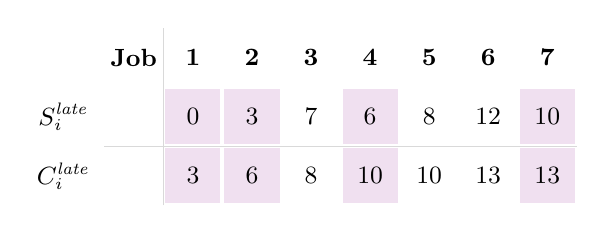
\begin{tikzpicture}[
    cell/.style={minimum width=7mm, minimum height=7mm,
                 font=\small, anchor=center},
    hdr/.style={cell, font=\small\bfseries},
    crit/.style={fill=violet!12},
    x=7.5mm, y=7.5mm
  ]
  % header
  \foreach \j/\lbl in {1/Job, 2/1, 3/2, 4/3, 5/4, 6/5, 7/6, 8/7} {
    \node[hdr] at (\j, 3) {\lbl};
  }
  % S_i^late
  \node[cell, font=\small\itshape] at (-0.2, 2) {$S_i^{\text{late}}$};
  \foreach \j/\v/\c in {2/0/crit, 3/3/crit, 4/7/, 5/6/crit, 6/8/, 7/12/, 8/10/crit} {
    \node[cell, \c] at (\j, 2) {\v};
  }
  % C_i^late
  \node[cell, font=\small\itshape] at (-0.2, 1) {$C_i^{\text{late}}$};
  \foreach \j/\v/\c in {2/3/crit, 3/6/crit, 4/8/, 5/10/crit, 6/10/, 7/13/, 8/13/crit} {
    \node[cell, \c] at (\j, 1) {\v};
  }
  % grid lines
  \draw[gray!30] (1.5, 0.5) -- (1.5, 3.5);
  \draw[gray!30] (0.5, 1.5) -- (8.5, 1.5);
\end{tikzpicture}
\caption{Latest start and completion times (CPM Backward).}
\label{fig:cpm-backward-table}
\end{figure}

\noindent
Tracing backwards from the sinks:
\begin{itemize}[nosep]
  \item Jobs~6 and~7 have no successors:
        $C_6^{\text{late}} = C_7^{\text{late}} = 13$.
        So $S_6^{\text{late}} = 12$, $S_7^{\text{late}} = 10$.
  \item Job~4: successors are 6 and 7.
        $C_4^{\text{late}} = \min(S_6^{\text{late}},
        S_7^{\text{late}}) = \min(12, 10) = 10$,
        $S_4^{\text{late}} = 6$.
  \item Job~5: successors are 6 and 7.
        $C_5^{\text{late}} = \min(12, 10) = 10$,
        $S_5^{\text{late}} = 8$.
  \item Job~2: successor is 4.
        $C_2^{\text{late}} = S_4^{\text{late}} = 6$,
        $S_2^{\text{late}} = 3$.
  \item Job~3: successor is 5.
        $C_3^{\text{late}} = S_5^{\text{late}} = 8$,
        $S_3^{\text{late}} = 7$.
  \item Job~1: successors are 2 and 3.
        $C_1^{\text{late}} = \min(3, 7) = 3$,
        $S_1^{\text{late}} = 0$.
\end{itemize}
\end{example}

% ------------------------------------------------------------
\subsection{The critical path}
\label{ssec:critical-path}
% ------------------------------------------------------------

\begin{definition}[Critical activity and critical path]
\label{def:critical-path}
A job~$i$ is \emph{critical} if its earliest and latest start
times coincide: $S_i = S_i^{\,\text{late}}$.
The \emph{critical path} is the set of all critical activities
(and the precedence arcs connecting them).
\end{definition}

A critical job has \emph{zero slack}: any delay in its execution
directly increases the makespan.  Non-critical jobs have
\emph{float}---they can shift within the interval
$[S_i,\; S_i^{\text{late}}]$ without affecting $\Cmax$.

\begin{example}[Critical path of the seven-job instance]
\label{ex:critical-path}
Comparing the forward and backward tables:

\medskip
\begin{center}
\begin{tabular}{lccccccc}
\toprule
\textbf{Job}             & 1 & 2 & 3 & 4 & 5 & 6 & 7 \\
\midrule
$S_i$ (earliest)         & 0 & 3 & 3 & 6 & 4 & 10 & 10 \\
$S_i^{\text{late}}$ (latest) & 0 & 3 & 7 & 6 & 8 & 12 & 10 \\
\midrule
Slack                    & 0 & 0 & 4 & 0 & 4 & 2  & 0 \\
Critical?                & \checkmark & \checkmark & & \checkmark & & & \checkmark \\
\bottomrule
\end{tabular}
\end{center}

\medskip\noindent
The critical path is $1 \to 2 \to 4 \to 7$, with
a total duration of $3 + 3 + 4 + 3 = 13 = \Cmax$.

\begin{figure}[H]
\centering
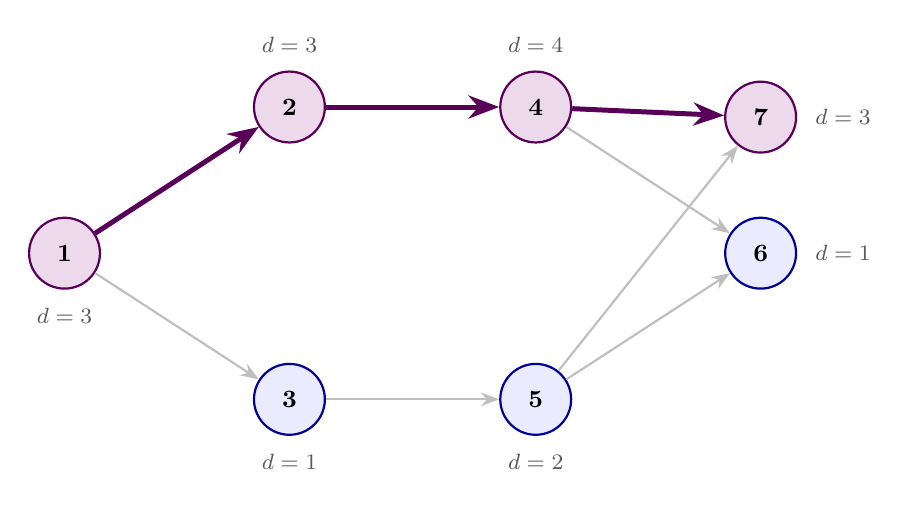
\begin{tikzpicture}[
    job/.style={circle, draw=blue!60!black, fill=blue!8,
                minimum size=9mm, font=\small\bfseries},
    cjob/.style={circle, draw=violet!70!black, fill=violet!15,
                 minimum size=9mm, font=\small\bfseries},
    dur/.style={font=\footnotesize, text=gray!70!black},
    ->, >=Stealth, thick, node distance=18mm and 22mm
  ]
  % critical nodes in violet
  \node[cjob] (1) {1};
  \node[cjob, above right=12mm and 22mm of 1] (2) {2};
  \node[job,  below right=12mm and 22mm of 1] (3) {3};
  \node[cjob, right=22mm of 2] (4) {4};
  \node[job,  right=22mm of 3] (5) {5};
  \node[job,  above right=12mm and 22mm of 5] (6) {6};
  \node[cjob, above=8mm of 6] (7) {7};

  % durations
  \node[dur, below=1mm of 1] {$d=3$};
  \node[dur, above=1mm of 2] {$d=3$};
  \node[dur, below=1mm of 3] {$d=1$};
  \node[dur, above=1mm of 4] {$d=4$};
  \node[dur, below=1mm of 5] {$d=2$};
  \node[dur, right=1mm of 6] {$d=1$};
  \node[dur, right=1mm of 7] {$d=3$};

  % critical arcs (violet, thicker)
  \draw[violet!70!black, line width=1.8pt] (1) -- (2);
  \draw[violet!70!black, line width=1.8pt] (2) -- (4);
  \draw[violet!70!black, line width=1.8pt] (4) -- (7);

  % non-critical arcs (gray)
  \draw[gray!50] (1) -- (3);
  \draw[gray!50] (3) -- (5);
  \draw[gray!50] (4) -- (6);
  \draw[gray!50] (5) -- (6);
  \draw[gray!50] (5) -- (7);
\end{tikzpicture}
\caption{The critical path $1 \to 2 \to 4 \to 7$
         (violet nodes and edges).
         Non-critical jobs and arcs are shown in gray.}
\label{fig:critical-path}
\end{figure}

\noindent
Job~3, for instance, can start anywhere between time~3 (earliest)
and time~7 (latest) without affecting the makespan.
Job~7, however, is locked: if it starts even one unit later, the
project finishes later.
\end{example}


% ------------------------------------------------------------
\subsection{Optimality of CPM}
\label{ssec:cpm-optimality}
% ------------------------------------------------------------

\begin{theorem}[CPM is optimal]
\label{thm:cpm-optimal}
The CPM Forward schedule achieves the minimum possible makespan
for the project scheduling problem
(\cref{def:project-scheduling}).
\end{theorem}

\begin{formaldetails}[Optimality of CPM]
The proof is by contradiction.
Consider the critical path $i_1 \to i_2 \to \cdots \to i_k$
found by CPM\@.
Every job on this path starts exactly when its predecessor
finishes (zero slack), so the makespan equals
\[
  \Cmax = d_{i_1} + d_{i_2} + \cdots + d_{i_k}.
\]
Any feasible schedule must respect the precedence chain
$i_1 \to i_2 \to \cdots \to i_k$, which means
\[
  \Cmax^* \;\ge\; d_{i_1} + d_{i_2} + \cdots + d_{i_k}
          \;=\; \Cmax.
\]
Since CPM produces a feasible schedule with makespan $\Cmax$,
and no feasible schedule can do better, CPM is optimal.
\qed
\end{formaldetails}

The key insight is that the critical path acts as a
\emph{lower bound}: no matter how cleverly we rearrange jobs,
we can never avoid executing every job on the critical path
in sequence, so the makespan is at least the sum of their
durations.  CPM \emph{achieves} this bound, so it is optimal.


% ============================================================
\section{Greedy Algorithms}
\label{sec:greedy-intro}
% ============================================================

CPM is our first example of a \textbf{greedy algorithm}.%
\aside{Italian: \emph{algoritmo avido};
the English ``greedy'' is standard.}

\begin{definition}[Greedy algorithm (informal)]
\label{def:greedy}
A greedy algorithm builds a solution incrementally.  At each step
it makes the locally best choice (assign the earliest possible
start time, pick the shortest job, etc.)\ and \emph{never
reconsiders} that choice.
\end{definition}

Greedy algorithms are typically very fast---often polynomial
time---because they never backtrack.  The catch is that for many
problems the locally best choice is not globally optimal.
CPM is a happy exception: the greedy ``start as early as possible''
rule happens to be provably optimal for the basic project
scheduling problem.

\begin{observation}
For more complex scheduling problems (with resources, deadlines,
or variable durations), greedy algorithms generally do \emph{not}
find the optimal solution.  We will need more powerful techniques:
enumeration, constraint programming, and local search.
\end{observation}


% ============================================================
\section{Algorithmic Analysis: Two Key Questions}
\label{sec:algo-analysis}
% ============================================================

Whenever we study a new algorithm, we ask two questions:

\begin{enumerate}
  \item \textbf{Computational complexity.}
    How does the running time scale with the input size?
    CPM processes each job once and inspects each precedence arc
    once, so its complexity is
    $\Oh{n + |P|}$%
    \aside{$|P|$ = number of arcs.  Worst case
    $\Oh{n^2}$; in practice graphs are
    sparse, so nearly linear.}---linear in the size of the input.

  \item \textbf{Exactness.}
    Does the algorithm always find the optimal solution?
    As we proved in \cref{thm:cpm-optimal}, CPM is \emph{exact}
    for the basic project scheduling problem.
\end{enumerate}

\begin{intermezzo}{CPM at scale}
In the lecture demo, a C++ implementation of CPM solved an
instance with \textbf{one million jobs} in about 4~seconds, and
instances with over 10~million jobs in under a minute.
The algorithm's simplicity---a single topological-order pass
through the DAG---translates directly into practical speed.
This is the power of a well-chosen greedy algorithm on a problem
where greedy happens to be optimal.
\end{intermezzo}


% ============================================================
\section{Instance Format}
\label{sec:instance-format}
% ============================================================

For the project scheduling problem we use a simple text format:%
\aside{Richer formats for more complex
problems; this suffices for the basic case.}

\begin{lstlisting}[language={}, caption={Instance file format
  for project scheduling.}, label={lst:ps-format}]
n                          (* number of jobs *)
d_1  #pred_1  pred_1a pred_1b ...
d_2  #pred_2  pred_2a pred_2b ...
...
d_n  #pred_n  pred_na pred_nb ...
\end{lstlisting}

\noindent
The first line gives the number of jobs~$n$.
Each subsequent line~$i$ (for $i = 1, \dots, n$) contains:
the duration~$d_i$, the number of predecessors, and the list of
predecessor indices.

\begin{example}[Instance file for \cref{ex:seven-jobs}]
\label{ex:instance-file}
\begin{lstlisting}[language={}, numbers=none]
7
3  0
3  1  1
1  1  1
4  1  2
2  1  3
1  2  4  5
3  2  4  5
\end{lstlisting}
Job~1 (line~2) has duration~3 and no predecessors.
Job~6 (line~7) has duration~1 and two predecessors: jobs~4 and~5.
\end{example}

% ============================================================
%  Lecture 2 — Knapsack, complexity, RCPSP, shop scheduling
%  (still Chapter 1: Introduction to Scheduling)
% ============================================================

\section{The Knapsack Problem}
\label{sec:knapsack}

Before continuing with scheduling problems, we take a detour
through a simpler combinatorial problem that lets us sharpen
three important ideas: greedy heuristics, upper bounds, and the
distinction between easy and hard problems.%
\aside{Not a scheduling problem, but the
perfect sandbox for greedy, bounds, and
complexity concepts.}

\begin{definition}[0/1 Knapsack Problem]
\label{def:knapsack}
We are given $n$ items, each with a \emph{weight} $w_i$ and a
\emph{value} $v_i$, and a knapsack of capacity~$W$.
We must choose a subset of items that fits in the knapsack
and maximises total value:
\[
  \max \sum_{i=1}^{n} v_i\, x_i
  \qquad\text{s.t.}\quad
  \sum_{i=1}^{n} w_i\, x_i \le W,
  \qquad x_i \in \{0,1\}.
\]
\end{definition}

In plain words: every item is either taken ($x_i = 1$) or
left behind ($x_i = 0$).  We want as much value as possible
without exceeding the weight limit.  Think of packing a
backpack for a hike, or---in computing---selecting files to
store on a disk with limited capacity.

% ------------------------------------------------------------
\subsection{Three greedy strategies}
\label{ssec:knapsack-greedy}
% ------------------------------------------------------------

\begin{example}[Six-item knapsack instance]
\label{ex:knapsack-six}
Consider six items with capacity $W = 100$:

\begin{figure}[H]
\centering
\begin{tabular}{lcccccc}
\toprule
\textbf{Item}   & 1   & 2   & 3   & 4  & 5  & 6 \\
\midrule
Weight $w_i$     & 100 & 50  & 45  & 20 & 10 & 5 \\
Value  $v_i$     & 40  & 35  & 18  & 4  & 10 & 2 \\
Ratio $v_i/w_i$  & 0.40& 0.70& 0.40& 0.20& 1.00& 0.40\\
\bottomrule
\end{tabular}
\caption{Data for the six-item knapsack instance
         (\cref{ex:knapsack-six}).}
\label{fig:knapsack-data}
\end{figure}
\end{example}

\noindent
Let's try three natural greedy rules on this instance:

\paragraph{Greedy 1: highest value first.}
Pick the item with the largest~$v_i$ that still fits.
\begin{itemize}[nosep]
  \item Select item~1 ($v = 40$, $w = 100$).
        Remaining capacity: $0$.
  \item No more items fit.
  \item \textbf{Total value: 40.}
\end{itemize}

\paragraph{Greedy 2: lightest first.}
Pick the item with the smallest~$w_i$ that still fits.
\begin{itemize}[nosep]
  \item Select item~6 ($w = 5$), then 5 ($w = 10$),
        then 4 ($w = 20$), then 3 ($w = 45$).
        Remaining capacity: $100 - 80 = 20$.
  \item Items~1 and~2 do not fit.
  \item \textbf{Total value: $2 + 10 + 4 + 18 = 34$.}
\end{itemize}

\paragraph{Greedy 3: best value-to-weight ratio.}
Pick the item with the highest $v_i / w_i$ that still fits.%
\aside{The classic knapsack heuristic.
Ties broken by largest item first.}
\begin{itemize}[nosep]
  \item Select item~5 (ratio 1.00, $w = 10$).
        Remaining: $90$.
  \item Select item~2 (ratio 0.70, $w = 50$).
        Remaining: $40$.
  \item Tied at ratio 0.40: items~1, 3, 6.
        Item~1 ($w = 100$) does not fit;
        item~3 ($w = 45$) does not fit;
        item~6 ($w = 5$) fits.  Remaining: $35$.
  \item Item~4 (ratio 0.20, $w = 20$) fits.  Remaining: $15$.
  \item \textbf{Total value: $10 + 35 + 2 + 4 = 51$.}
        Weight used: $85$.
\end{itemize}

\medskip\noindent
None of these finds the optimal solution.  By inspection, items
$\{2, 3, 6\}$ weigh exactly $50 + 45 + 5 = 100$ and achieve
value $35 + 18 + 2 = \mathbf{55}$.  The best greedy (ratio-based)
left 15 units of capacity unused, missing a better packing.

% ------------------------------------------------------------
\subsection{Upper bounds via relaxation}
\label{ssec:knapsack-bound}
% ------------------------------------------------------------

We found a solution worth~55 by inspection, but how do we
\emph{prove} no solution can do better?  The standard technique
is \emph{relaxation}: solve an easier version of the problem
whose optimal value is guaranteed to be at least as good.%
\aside{For a maximisation problem, a relaxation gives an
\emph{upper bound}.  For minimisation (like makespan), it gives
a \emph{lower bound}.}

\begin{definition}[Fractional Knapsack]
\label{def:fractional-knapsack}
The same formulation as \cref{def:knapsack}, but with
$x_i \in [0, 1]$ instead of $x_i \in \{0, 1\}$.
Items may be taken in fractions: if only half of item~$i$
fits, we take half and get $\tfrac{1}{2} v_i$.
\end{definition}

Since any 0/1 solution is also a valid fractional solution,
the fractional optimum is an upper bound on the integer optimum.
And the fractional problem has a simple exact greedy:

\begin{observation}
The greedy algorithm that sorts items by decreasing $v_i / w_i$
and takes as much of each item as fits is \emph{optimal}
for the fractional knapsack.
\end{observation}

\begin{example}[Fractional bound for \cref{ex:knapsack-six}]
\label{ex:fractional-bound}
Sort by ratio: item~5 (1.00), item~2 (0.70), then the
0.40-ratio group.
\begin{itemize}[nosep]
  \item Take all of item~5: weight 10, value 10. Remaining: 90.
  \item Take all of item~2: weight 50, value 35. Remaining: 40.
  \item Item~1 weighs 100; take $40/100 = 0.4$ of it:
        weight 40, value $0.4 \times 40 = 16$.
        Remaining: 0.
\end{itemize}
Total value: $10 + 35 + 16 = \mathbf{61}$.
Since the integer optimum $\le 61$ and we found a feasible
integer solution worth~55, the optimality gap is at most
$61 - 55 = 6$.
\end{example}

\begin{remark}
The fractional bound does not prove that 55 is optimal
(there could be an integer solution worth 56, 57, \ldots, 61).
For this small instance we verified optimality by inspection.
For large instances, tighter bounds or exact algorithms
(branch-and-bound, dynamic programming) are needed.
\end{remark}


% ============================================================
\section{Easy vs Hard Problems}
\label{sec:easy-hard}
% ============================================================

So far we have seen two \emph{easy} problems---project scheduling
and fractional knapsack---where a greedy algorithm finds the
optimum in polynomial time.  The 0/1 knapsack, by contrast,
is \emph{hard}: no known polynomial-time algorithm solves it
exactly.

\begin{definition}[$\NP$-hard (informal)]
\label{def:np-hard-informal}
A problem is $\NP$-hard if the best known exact algorithms
require time exponential in the input size.%
\aside{Whether $\NP$-hard problems truly
require exponential time is the open
$\mathsf{P} \stackrel{?}{=} \NP$ question.}
\end{definition}

The key structural difference: for easy problems, the algorithm
makes locally optimal choices with no branching.  For hard
problems, at each step there are multiple choices (which item
to take, which job to schedule next), and exploring all
combinations leads to an exponential number of candidate
solutions---roughly $2^n$ for $n$ binary decisions.

\begin{figure}[H]
\centering
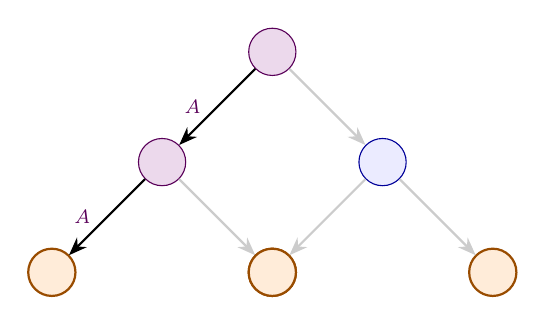
\begin{tikzpicture}[
    level distance=14mm, sibling distance=28mm,
    edge from parent/.style={draw, -Stealth, thick},
    every node/.style={circle, draw=blue!60!black, fill=blue!8,
                       minimum size=6mm, font=\footnotesize},
    leaf/.style={fill=orange!15, draw=orange!60!black},
    chosen/.style={fill=violet!15, draw=violet!70!black},
    grayedge/.style={draw=gray!40, -Stealth},
    >=Stealth
  ]
  \node[chosen] {}
    child { node[chosen] {}
      child { node[chosen, leaf] {}
        edge from parent node[left, draw=none, fill=none,
          font=\scriptsize\itshape, text=violet!70!black] {A} }
      child { node[leaf] {}
        edge from parent[grayedge] }
      edge from parent node[left, draw=none, fill=none,
        font=\scriptsize\itshape, text=violet!70!black] {A} }
    child { node {}
      child { node[leaf] {}
        edge from parent[grayedge] }
      child { node[leaf] {}
        edge from parent[grayedge] }
      edge from parent[grayedge] };
\end{tikzpicture}
\caption{A greedy algorithm (violet path) picks one branch at
         each decision point, visiting $n$ nodes total.
         An exact algorithm may need to explore all $2^n$
         leaves.}
\label{fig:search-tree}
\end{figure}

\noindent
A \textbf{greedy} algorithm traverses a single root-to-leaf path
through this tree: fast ($n$~steps), but no guarantee of finding
the best leaf.
An \textbf{exact} algorithm explores enough of the tree to
certify optimality---potentially all of it.

\begin{observation}
Algorithms fall into two families:
\begin{itemize}[nosep]
  \item \textbf{Exact} algorithms guarantee the optimal
        solution, but may take exponential time on hard problems.
  \item \textbf{Heuristic} algorithms (greedy being the simplest
        subfamily) find good solutions quickly, without optimality
        guarantees.
\end{itemize}
This course covers both: we will implement greedy heuristics,
enumeration (backtracking), constraint programming (via MiniZinc),
and local search / metaheuristics.
\end{observation}


% ============================================================
\section{Resource-Constrained Project Scheduling (RCPSP)}
\label{sec:rcpsp}
% ============================================================

We now return to project scheduling and add the complication we
set aside earlier: \textbf{resources}.

\begin{definition}[Resource-Constrained Project Scheduling
  Problem---RCPSP]
\label{def:rcpsp}
We are given the same data as the basic project scheduling
problem (\cref{def:project-scheduling}), plus:
\begin{itemize}[nosep]
  \item $R$ types of \emph{renewable resources}, each with a
        capacity $Q_r$ ($r = 1, \dots, R$);
  \item for each job~$i$ and resource~$r$, the
        \emph{resource demand} $q_{ir}$: how many units of
        resource~$r$ job~$i$ uses while executing.
\end{itemize}
Resources are \emph{renewable}: a unit is occupied while a job
runs, then becomes available again.%
\aside{Workers, machines: busy during the
job, free afterwards.  Non-renewable
resources are consumed permanently.}

\medskip\noindent
A schedule must satisfy:
\begin{enumerate}[nosep]
  \item all precedence constraints (as before);
  \item at every time instant~$t$, the total demand for each
        resource~$r$ from all jobs running at time~$t$ does not
        exceed $Q_r$.
\end{enumerate}
The objective is to minimise the makespan $\Cmax$.
\end{definition}

The resource constraints are what make RCPSP fundamentally harder
than basic project scheduling.  Without resources, CPM schedules
every job as early as possible---there is no conflict.  With
resources, two jobs may both be ready to start, but starting
them simultaneously would exceed a resource capacity.  We must
choose which one goes first, and that choice affects all
subsequent decisions.

\begin{example}[RCPSP with two resources]
\label{ex:rcpsp-seven}
Take the seven-job instance from \cref{ex:seven-jobs} and add
two resources with capacities $Q_1 = 4$, $Q_2 = 3$:

\begin{figure}[H]
\centering
\begin{tabular}{lccccccc}
\toprule
\textbf{Job}      & 1 & 2 & 3 & 4 & 5 & 6 & 7 \\
\midrule
Duration $d_i$     & 3 & 3 & 1 & 4 & 2 & 1 & 3 \\
$q_{i,1}$ (R1)     & 3 & 2 & 3 & 1 & 0 & 2 & 1 \\
$q_{i,2}$ (R2)     & 0 & 2 & 1 & 2 & 2 & 1 & 2 \\
\bottomrule
\end{tabular}
\caption{Resource demands for the seven-job RCPSP instance.}
\label{fig:rcpsp-data}
\end{figure}

\noindent
With CPM (ignoring resources), jobs~2 and~3 start simultaneously
at time~3.  But job~2 needs 2~units of R1 and job~3 needs 3:
together that is $2 + 3 = 5 > 4 = Q_1$.  They cannot run in
parallel---we must choose.  This is a \textbf{choice point} that
does not exist in the unconstrained version.
\end{example}

% ------------------------------------------------------------
\subsection{Why RCPSP is hard}
\label{ssec:rcpsp-hard}
% ------------------------------------------------------------

Each choice point roughly doubles the number of candidate
schedules.  With $n$~jobs, the search space grows to approximately
$2^n$ alternatives.%
\aside{$2^n$ is a rough upper bound; the
true number depends on the graph
and resource constraints.}
For $n = 100$, that is $2^{100} \approx 10^{30}$
schedules---impossible to enumerate.

RCPSP is $\NP$-hard.  The PSPlib benchmark library contains
instances with 30, 60, 90, and 120~jobs;
some 120-job instances remain \emph{unsolved to optimality}
to this day.

% ------------------------------------------------------------
\subsection{Lower bound for RCPSP}
\label{ssec:rcpsp-lower-bound}
% ------------------------------------------------------------

A natural lower bound: \textbf{ignore the resource constraints}
and solve the resulting basic project scheduling problem with CPM\@.
Since removing constraints can only improve (or maintain) the
optimal value:
\[
  \Cmax^{\text{CPM}} \;\le\; \Cmax^{\text{RCPSP}*}.
\]
If a heuristic solution happens to match this bound, we know it
is optimal.  Otherwise, the gap
$\Cmax^{\text{heuristic}} - \Cmax^{\text{CPM}}$
tells us how far we \emph{might} be from optimality (though the
true optimum could lie anywhere in between).

% ------------------------------------------------------------
\subsection{Greedy heuristics for RCPSP}
\label{ssec:rcpsp-greedy}
% ------------------------------------------------------------

A greedy heuristic for RCPSP extends the CPM idea:
schedule one job at a time, choosing the \emph{earliest feasible}
start that respects both precedences and resources.
The question is: \textbf{which job to schedule next?}

There are two main families of greedy rules:

\paragraph{Time-based (schedule generation scheme).}
Advance time instant by instant.  At each moment, identify all
jobs that \emph{could} start (predecessors done, resources
available) and pick one by a priority rule:
longest processing time, shortest processing time, most resource
demand, etc.

\paragraph{Job-based (priority rule).}
Maintain three sets:
\begin{itemize}[nosep]
  \item \emph{Scheduled}: jobs already placed.
  \item \emph{Ready}: jobs whose predecessors are all scheduled.
  \item \emph{Not ready}: at least one predecessor is unscheduled.
\end{itemize}
At each step, select a job from the \emph{ready} set by a
priority rule, then find the earliest time at which it can start
without violating resource capacities.

\begin{remark}
Because the greedy traverses a single path through the exponential
search tree, different runs with different priority rules---or
even random tie-breaking---can produce very different makespans.
In the seven-job example, random restarts yielded solutions
ranging from $\Cmax = 14$ to $\Cmax = 16$, against a CPM lower
bound of~12.
\end{remark}

% ------------------------------------------------------------
\subsection{RCPSP extensions}
\label{ssec:rcpsp-extensions}
% ------------------------------------------------------------

Several extensions make the problem richer (and harder):

\begin{itemize}
  \item \textbf{Multi-mode RCPSP.}
    Each job has several \emph{execution modes}, each with its own
    duration and resource demands.
    For instance, digging a trench might take 3~days with
    3~workers, or 2~days with 1~worker and an excavator.
    The decision now includes both \emph{when} and \emph{how}
    to execute each job.

  \item \textbf{Non-renewable resources.}
    Resources that are \emph{consumed} (concrete, fuel, budget).
    In the single-mode case, total consumption is fixed regardless
    of schedule---feasibility reduces to checking whether the
    total demand exceeds supply.  Combined with multiple modes,
    however, the choice of mode affects consumption, making the
    problem significantly harder.

  \item \textbf{Preemption.}
    A job may be \emph{interrupted} and resumed later, freeing
    its resources for another job in the meantime.
    Whether preemption is realistic depends on the application:
    pausing a software build is easy; pausing a concrete pour
    is not.

  \item \textbf{Stochastic durations.}
    Durations drawn from probability distributions.
    Objectives become expected or worst-case makespan---this
    variant belongs more to the Project Management course.
\end{itemize}


% ============================================================
\section{Shop Scheduling Problems}
\label{sec:shop-scheduling}
% ============================================================

We now introduce a family of scheduling problems where
\emph{machines} (processors) are the central resource.
These are called \textbf{shop scheduling} problems.%
\aside{``Shop'' = workshop/factory floor,
not a retail store.}

The common setup: we have $n$ \emph{jobs} and $m$
\emph{machines}.  Each job consists of a sequence of
\emph{tasks} (also called \emph{operations}), where each task
must be processed on a specific machine for a given duration.
A machine can process at most one task at a time, and
(unless stated otherwise) a task cannot be interrupted once started.

% ------------------------------------------------------------
\subsection{Job Shop Scheduling (JSS)}
\label{ssec:job-shop}
% ------------------------------------------------------------

\begin{definition}[Job Shop Scheduling Problem]
\label{def:job-shop}
We are given:
\begin{itemize}[nosep]
  \item $n$ jobs, each consisting of an \emph{ordered} sequence
        of tasks;
  \item $m$ machines;
  \item each task $T_{ij}$ (the $j$-th task of job~$i$) is
        assigned to a specific machine $\mu_{ij}$ and has
        duration $d_{ij}$;
  \item (optionally) a \emph{release date} $r_i$ and a
        \emph{due date} $\bar{d}_i$ for each job.
\end{itemize}
\textbf{Constraints:}
\begin{enumerate}[nosep]
  \item \emph{Precedence within each job:} the tasks of a job
        must be processed in their given order.
  \item \emph{Machine capacity:} each machine processes at most
        one task at a time.
  \item Release dates are hard constraints.
\end{enumerate}
\textbf{Objective:} minimise the makespan $\Cmax$, or minimise
total \emph{tardiness} $\sum_i T_i$, where
$T_i = \max(0,\; C_i - \bar{d}_i)$ is the delay of job~$i$
past its due date.
\end{definition}

\begin{example}[A small job shop]
\label{ex:job-shop-small}
Three jobs on three machines:

\begin{figure}[H]
\centering
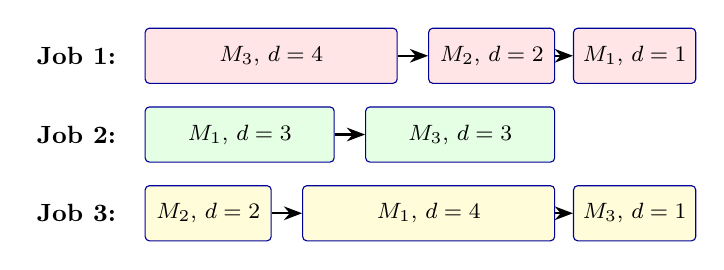
\begin{tikzpicture}[
    task/.style={draw=blue!60!black, fill=blue!8,
                 minimum height=7mm, font=\small,
                 rounded corners=1.5pt, anchor=west},
    arr/.style={-Stealth, thick},
    mlab/.style={font=\small\bfseries, anchor=east},
    x=8mm, y=10mm
  ]
  % Job 1: M3 -> M2 -> M1
  \node[mlab] at (-0.3, 3) {Job 1:};
  \node[task, fill=red!10, minimum width=32mm] (j1t1) at (0, 3)
    {\footnotesize $M_3$, $d=4$};
  \node[task, fill=red!10, minimum width=16mm] (j1t2) at (4.5, 3)
    {\footnotesize $M_2$, $d=2$};
  \node[task, fill=red!10, minimum width=8mm] (j1t3) at (6.8, 3)
    {\footnotesize $M_1$, $d=1$};
  \draw[arr] (j1t1) -- (j1t2);
  \draw[arr] (j1t2) -- (j1t3);

  % Job 2: M1 -> M3
  \node[mlab] at (-0.3, 2) {Job 2:};
  \node[task, fill=green!10, minimum width=24mm] (j2t1) at (0, 2)
    {\footnotesize $M_1$, $d=3$};
  \node[task, fill=green!10, minimum width=24mm] (j2t2) at (3.5, 2)
    {\footnotesize $M_3$, $d=3$};
  \draw[arr] (j2t1) -- (j2t2);

  % Job 3: M2 -> M1 -> M3
  \node[mlab] at (-0.3, 1) {Job 3:};
  \node[task, fill=yellow!15, minimum width=16mm] (j3t1) at (0, 1)
    {\footnotesize $M_2$, $d=2$};
  \node[task, fill=yellow!15, minimum width=32mm] (j3t2) at (2.5, 1)
    {\footnotesize $M_1$, $d=4$};
  \node[task, fill=yellow!15, minimum width=8mm] (j3t3) at (6.8, 1)
    {\footnotesize $M_3$, $d=1$};
  \draw[arr] (j3t1) -- (j3t2);
  \draw[arr] (j3t2) -- (j3t3);
\end{tikzpicture}
\caption{Three jobs in a job shop.  Each row shows one job's
         task sequence with its assigned machine and duration.
         Arrows indicate precedence within the job.}
\label{fig:job-shop-example}
\end{figure}

\noindent
Job~1 visits machines $3 \to 2 \to 1$; job~2 visits $1 \to 3$;
job~3 visits $2 \to 1 \to 3$.
The scheduler must decide, for each machine, in what order to
process the tasks assigned to it---without violating the
within-job precedences.
\end{example}

% ------------------------------------------------------------
\subsection{Flow Shop Scheduling (FSS)}
\label{ssec:flow-shop}
% ------------------------------------------------------------

\begin{definition}[Flow Shop Scheduling Problem]
\label{def:flow-shop}
A special case of the job shop where \textbf{all jobs visit the
machines in the same fixed order} $M_1 \to M_2 \to \cdots \to M_m$.
Every job has exactly $m$~tasks (some may have duration zero).
\end{definition}

The crucial simplification: since the machine order is
identical for every job, the \emph{only} decision is the
\textbf{permutation} (sequence) in which jobs enter the shop.%
\aside{If all machines use the same permutation, we have a
\emph{permutation flow shop}---the most common variant.}
Once the permutation is fixed, start times follow
deterministically: each task starts as soon as both its machine
is free and the previous task of the same job is finished.

\begin{figure}[H]
\centering
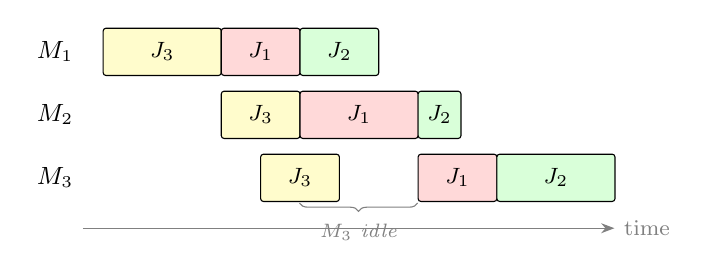
\begin{tikzpicture}[
    x=5mm, y=8mm,
    block/.style={draw, minimum height=6mm,
                  rounded corners=1pt, anchor=west,
                  font=\footnotesize},
    mlab/.style={font=\small\bfseries, anchor=east}
  ]
  % Machine labels
  \node[mlab] at (-0.5, 3) {$M_1$};
  \node[mlab] at (-0.5, 2) {$M_2$};
  \node[mlab] at (-0.5, 1) {$M_3$};

  % Job 3 (first in permutation)
  \node[block, fill=yellow!20, minimum width=15mm]
    (j3m1) at (0, 3) {$J_3$};
  \node[block, fill=yellow!20, minimum width=10mm]
    (j3m2) at (3, 2) {$J_3$};
  \node[block, fill=yellow!20, minimum width=10mm]
    (j3m3) at (4, 1) {$J_3$};

  % Job 1 (second)
  \node[block, fill=red!15, minimum width=10mm]
    (j1m1) at (3, 3) {$J_1$};
  \node[block, fill=red!15, minimum width=15mm]
    (j1m2) at (5, 2) {$J_1$};
  \node[block, fill=red!15, minimum width=10mm]
    (j1m3) at (8, 1) {$J_1$};

  % Job 2 (third)
  \node[block, fill=green!15, minimum width=10mm]
    (j2m1) at (5, 3) {$J_2$};
  \node[block, fill=green!15, minimum width=5mm]
    (j2m2) at (8, 2) {$J_2$};
  \node[block, fill=green!15, minimum width=15mm]
    (j2m3) at (10, 1) {$J_2$};

  % idle gap annotation
  \draw[decorate, decoration={brace, amplitude=3pt, mirror},
        gray]
    (5, 0.6) -- (8, 0.6)
    node[midway, below=4pt, font=\scriptsize\itshape, text=gray]
    {$M_3$ idle};

  % time axis
  \draw[-Stealth, gray] (-0.5, 0.2) -- (13, 0.2)
    node[right, font=\footnotesize] {time};
\end{tikzpicture}
\caption{A flow shop Gantt chart for the permutation
         $J_3, J_1, J_2$.  Machine~$M_3$ sits idle between
         $J_3$ and~$J_1$ because it must wait for $J_1$ to
         finish on~$M_2$.  A different permutation might reduce
         this idle time.}
\label{fig:flow-shop-gantt}
\end{figure}

\noindent
The goal is to find the permutation that minimises idle gaps and
thus the makespan.  Despite this structural simplification, the
flow shop with $m \ge 3$ machines is $\NP$-hard.

% ------------------------------------------------------------
\subsection{Open Shop Scheduling (OSS)}
\label{ssec:open-shop}
% ------------------------------------------------------------

\begin{definition}[Open Shop Scheduling Problem]
\label{def:open-shop}
Like the job shop, but with \textbf{no fixed ordering} of tasks
within a job.  Each job still has one task per machine, but the
scheduler is free to choose in which order a job visits the
machines.
\end{definition}

In the open shop, the within-job precedences disappear entirely.
What ties a job's tasks together are its release date and due
date: all tasks of a job must start after its release and finish
before its deadline.  The scheduler must decide both the
\emph{order of tasks within each job} and the \emph{order of
jobs on each machine}.

\medskip
\begin{center}
\begin{tabular}{lccc}
\toprule
 & \textbf{Machine order} & \textbf{Decision variable}
 & \textbf{Complexity} \\
\midrule
Job shop  & job-specific, fixed
          & start time of each task
          & $\NP$-hard \\
Flow shop & same for all jobs
          & job permutation
          & $\NP$-hard ($m \ge 3$) \\
Open shop & free
          & task order + start times
          & $\NP$-hard ($m \ge 3$) \\
\bottomrule
\end{tabular}
\end{center}

\begin{intermezzo}{Make as a project scheduler}
When you type \texttt{make} to compile a C++ project, the build
tool reads the dependency graph from the Makefile and solves a
project scheduling problem: each compilation command is a job,
its duration is the compilation time, and ``\texttt{A.o} depends
on \texttt{A.cc}'' is a precedence constraint.

With \texttt{make -j} (parallel mode), Make schedules independent
compilations on separate CPU cores---exactly the CPM forward
strategy.  In a classroom demo, a synthetic Makefile encoding the
seven-job instance from \cref{ex:seven-jobs} (using \texttt{sleep}
to simulate durations) completed in 12~seconds with
\texttt{make -j}, matching the CPM makespan, versus 16~seconds
in sequential mode.
\end{intermezzo}

% ============================================================
%  Lecture 3 — Graph coloring, timetabling, sport scheduling
%  (still Chapter 1: Introduction to Scheduling)
% ============================================================

\section{Graph Colouring}
\label{sec:graph-colouring}

Many scheduling and timetabling problems reduce, at their core,
to assigning \emph{labels} (colours) to objects so that
conflicting objects receive different labels.  This is precisely
the \textbf{graph colouring} problem.%
\aside{Applications: register allocation,
frequency assignment, map colouring.}

\begin{definition}[Graph Colouring---two formulations]
\label{def:graph-colouring}
Given an undirected graph $G = (V, E)$:
\begin{enumerate}[nosep]
  \item \textbf{Search version.}
    Given an integer $k$, find a \emph{proper $k$-colouring}:
    an assignment $c\colon V \to \{1,\dots,k\}$ such that
    $c(u) \neq c(v)$ for every edge $\{u,v\} \in E$.
  \item \textbf{Optimisation version.}
    Find the minimum $k$ for which a proper $k$-colouring exists.
    This minimum is the \emph{chromatic number} $\chi(G)$.
\end{enumerate}
\end{definition}

The search version asks: ``can I do it with $k$ colours?''
The optimisation version asks: ``what is the fewest colours I
need?''  Both are $\NP$-hard in general (for $k \ge 3$).

% ------------------------------------------------------------
\subsection{Greedy colouring}
\label{ssec:greedy-colouring}
% ------------------------------------------------------------

The simplest approach: process vertices one by one and assign each
the \emph{smallest colour not used by its already-coloured
neighbours}.  The quality depends entirely on the \textbf{vertex
ordering}.

\paragraph{Maximum-degree ordering.}
Sort vertices by decreasing degree (number of neighbours) and
colour in that order.  The intuition: high-degree vertices are
the most constrained, so handle them first while many colours
are still available.

\begin{example}[Greedy colouring by max degree]
\label{ex:greedy-colour-maxdeg}
Consider a graph on five vertices:

\begin{figure}[H]
\centering
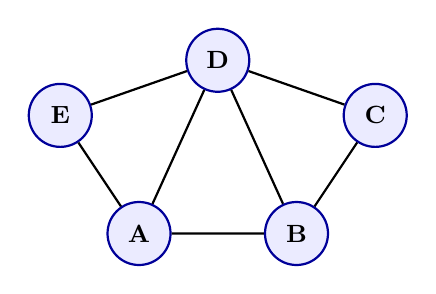
\begin{tikzpicture}[
    vtx/.style={circle, draw=blue!60!black, fill=blue!8,
                minimum size=8mm, font=\small\bfseries},
    >=Stealth, thick
  ]
  \node[vtx] (a) at (0, 0)   {A};
  \node[vtx] (b) at (2, 0)   {B};
  \node[vtx] (c) at (3, 1.5) {C};
  \node[vtx] (d) at (1, 2.2) {D};
  \node[vtx] (e) at (-1, 1.5){E};
  \draw (a)--(b) (a)--(d) (a)--(e)
        (b)--(c) (b)--(d)
        (c)--(d)
        (d)--(e);
\end{tikzpicture}
\caption{A small graph.  Vertex~D has the highest degree (4),
         followed by A and B (degree~3 each).}
\label{fig:greedy-colour-graph}
\end{figure}

\noindent
Degrees: $D = 4$, $A = 3$, $B = 3$, $C = 2$, $E = 2$.
Processing in order $D, A, B, C, E$:
\begin{enumerate}[nosep]
  \item $D$: no coloured neighbours $\Rightarrow$ colour~1.
  \item $A$: neighbour $D$ has colour~1 $\Rightarrow$ colour~2.
  \item $B$: neighbours $D$(1), $A$(2) $\Rightarrow$ colour~3.
  \item $C$: neighbours $B$(3), $D$(1) $\Rightarrow$ colour~2.
  \item $E$: neighbours $A$(2), $D$(1) $\Rightarrow$ colour~3.
\end{enumerate}
Result: 3 colours.  In fact $\chi(G) = 3$ here, so the greedy
found the optimum---but this is not guaranteed in general.
\end{example}

% ------------------------------------------------------------
\subsection{DSatur}
\label{ssec:dsatur}
% ------------------------------------------------------------

A smarter ordering is \textbf{DSatur}
(Degree of Saturation),%
\aside{Br\'{e}laz, 1979.  Still competitive
with far more complex heuristics.}
which chooses the next vertex \emph{dynamically} rather than
fixing the order upfront.

\begin{definition}[Saturation degree]
\label{def:saturation-degree}
The \emph{saturation degree} of a vertex~$v$ is the number of
\emph{distinct colours} already assigned to its neighbours.
\end{definition}

\begin{definition}[DSatur algorithm]
\label{def:dsatur}
Repeat until all vertices are coloured:
\begin{enumerate}[nosep]
  \item Among uncoloured vertices, pick the one with the
        \textbf{highest saturation degree}.
        Break ties by highest (uncoloured) degree; break further
        ties arbitrarily.
  \item Assign it the smallest colour not used by its neighbours.
\end{enumerate}
\end{definition}

The intuition: a vertex with high saturation is surrounded by
many different colours, so it is the most ``urgent'' to colour
next---it has the fewest options left.  By always attending to the
most constrained vertex, DSatur avoids wasteful colour
introductions more often than a static ordering.

\begin{example}[DSatur on the same graph]
\label{ex:dsatur}
Using the graph from \cref{fig:greedy-colour-graph}:
\begin{enumerate}[nosep]
  \item All saturations are 0; pick $D$ (highest degree~4)
        $\Rightarrow$ colour~1.
  \item Saturations: $A = 1$, $B = 1$, $C = 1$, $E = 1$.
        Tie; pick $A$ (degree~3) $\Rightarrow$ colour~2.
  \item Saturations: $B = 2$, $C = 1$, $E = 2$.
        Tie between $B$ and $E$; pick $B$ (degree~3)
        $\Rightarrow$ colour~3.
  \item Saturations: $C = 2$, $E = 2$.
        Tie; pick $C$ (degree~2) $\Rightarrow$ colour~2.
  \item $E$: saturation~2 $\Rightarrow$ colour~3.
\end{enumerate}
Same result (3 colours), but on larger graphs DSatur typically
outperforms static max-degree ordering.
\end{example}

\begin{remark}
DSatur is exact for bipartite graphs (always finds $\chi = 2$)
and for cycle graphs.  For general graphs it is a heuristic:
it may use more than $\chi(G)$ colours.
\end{remark}


% ============================================================
\section{Timetabling Problems}
\label{sec:timetabling}
% ============================================================

Timetabling is the task of assigning events (exams, lectures,
shifts, matches) to time slots and resources (rooms, people,
fields) subject to a rich set of constraints.%
\aside{At their core, timetabling =
graph colouring with richer
constraints.}

We survey three major families: educational, workforce, and
sport timetabling.

% ------------------------------------------------------------
\subsection{Educational timetabling}
\label{ssec:educational-timetabling}
% ------------------------------------------------------------

\paragraph{Examination timetabling.}
Assign exams to time slots so that no student has two exams at
the same time.  The conflict graph has one vertex per exam and an
edge whenever two exams share at least one enrolled student.
The problem then reduces to graph colouring (minimise the number
of time slots, or fit within a given number).  Additional soft
constraints typically include:
\begin{itemize}[nosep]
  \item spreading each student's exams over the available days
        (avoid two exams on the same day or on consecutive days);
  \item room capacity limits;
  \item preferred time slots for large exams.
\end{itemize}

\paragraph{Course timetabling.}
Assign lectures to weekly time slots and rooms.
The \emph{curriculum-based} variant%
\aside{Central to ITC-2007, Track~3.}
defines conflicts not by individual enrolments but by
\emph{curricula}: pre-defined groups of courses that share
students.  Two courses in the same curriculum cannot be scheduled
at the same time.

\begin{definition}[Curriculum-Based Course Timetabling
  (CB-CTT, simplified)]
\label{def:cb-ctt}
Given:
\begin{itemize}[nosep]
  \item a set of courses, each with a number of weekly lectures,
        a teacher, and membership in one or more curricula;
  \item a set of rooms, each with a capacity;
  \item a set of time slots (periods $\times$ days);
  \item teacher unavailability constraints.
\end{itemize}
Hard constraints:
\begin{enumerate}[nosep]
  \item[H1.] No two lectures of courses in the same curriculum
             at the same time.
  \item[H2.] No teacher teaches two courses at the same time.
  \item[H3.] Room capacity is respected.
  \item[H4.] Each course gets exactly its required number of
             lectures.
\end{enumerate}
Soft constraints (penalised in the objective):
\begin{enumerate}[nosep]
  \item[S1.] Room stability: a course should use the same room
             across all its lectures.
  \item[S2.] Minimum working days: lectures of a course should
             be spread over a minimum number of days.
  \item[S3.] Curriculum compactness: lectures of the same
             curriculum on the same day should be in adjacent
             time slots (no ``holes'' in a student's schedule).
\end{enumerate}
\end{definition}

\paragraph{High-school timetabling.}
Similar to course timetabling, but typically with tighter
constraints: each class has a fixed weekly schedule, teachers
must not have gaps between lessons, and there may be requirements
on the distribution of subjects throughout the week
(e.g.\ no more than two hours of maths per day).

% ------------------------------------------------------------
\subsection{Workforce timetabling: nurse rostering}
\label{ssec:nurse-rostering}
% ------------------------------------------------------------

Workforce timetabling assigns employees to shifts over a planning
horizon, balancing coverage requirements with labour regulations
and personal preferences.  The most studied instance is the
\textbf{nurse rostering problem} (NRP).

\begin{definition}[Nurse Rostering Problem (simplified)]
\label{def:nurse-rostering}
Given:
\begin{itemize}[nosep]
  \item a set of \emph{nurses}, each with a \emph{contract}
        (min/max working days, complete-weekend flag) and a set
        of \emph{skills} (head nurse, regular nurse, trainee,
        \ldots);
  \item a set of \emph{shift types} (Early, Late, Night, \ldots)
        with forbidden successions (e.g.\ Night $\to$ Early is
        not allowed);
  \item for each (shift, skill, day) triple, a \emph{minimum}
        and \emph{optimal} staffing requirement;
  \item a set of nurse \emph{shift-off requests}: preferred
        days off or shifts to avoid.
\end{itemize}
A solution assigns each nurse, for each day of the planning
horizon (typically one week), either a (shift, skill) pair or a
day off.
\end{definition}

\paragraph{Constraints.}
Hard constraints must always be satisfied:
\begin{enumerate}[nosep]
  \item[H1.] \emph{Single assignment:} at most one shift per
             nurse per day.
  \item[H2.] \emph{Minimum staffing:} each (shift, skill, day)
             must meet the minimum requirement.
  \item[H3.] \emph{Shift successions:} no forbidden
             day-to-day shift sequences.
  \item[H4.] \emph{Skill matching:} a nurse can only cover a
             skill she possesses.
\end{enumerate}

\noindent
Soft constraints contribute to the objective function
(lower is better), each weighted:
\begin{enumerate}[nosep]
  \item[S1.] \emph{Optimal coverage} (weight~3):
             each nurse below the optimal requirement is penalised.
  \item[S2.] \emph{Preferences} (weight~1):
             each assignment to an undesired shift is penalised.
  \item[S3.] \emph{Complete weekend} (weight~3):
             if flagged, the nurse should work both Sat and Sun or
             neither.
  \item[S4.] \emph{Total assignments} (weight~2):
             working days outside the contract's $[\min, \max]$
             range are penalised.
\end{enumerate}

\begin{example}[NR-05: a five-nurse instance]
\label{ex:nr-05}
The smallest benchmark instance has 5~nurses, 2~skills, 3~shift
types, and a one-week horizon.  The instance file follows a
structured text format:

\begin{lstlisting}[language={}, numbers=none,
  caption={Excerpt from the NR-05 instance file.}]
SKILLS = 2
HeadNurse
Nurse

SHIFT_TYPES = 3
Early 0
Late 1 Early
Night 2 Early Late

CONTRACTS = 2
FullTime (4,5) 1
PartTime (2,3) 1

NURSES = 5
Patrick FullTime 2 HeadNurse Nurse
Andrea  FullTime 2 HeadNurse Nurse
Stefaan PartTime 2 HeadNurse Nurse
Sara    PartTime 1 Nurse
Nguyen  FullTime 1 Nurse
\end{lstlisting}

\noindent
A solution is a list of (nurse, day, shift, skill) assignments.
Benchmark instances with 12, 21, 30, 40, 50, 60, and 80 nurses
are available in the course materials.%
\aside{Derived from INRC-II.}
\end{example}


% ------------------------------------------------------------
\subsection{Sport timetabling: round-robin tournaments}
\label{ssec:sport-timetabling}
% ------------------------------------------------------------

In a \emph{round-robin tournament}, every team plays every
other team exactly once (single round-robin) or twice
(double round-robin, with home and away legs).
The scheduling problem: assign matches to \emph{rounds}
(time slots) so that each team plays exactly once per round,
while respecting venue constraints (home/away balance, travel
minimisation, broadcaster requests, etc.).

\paragraph{Canonical $\mathbf{1}$-factorisation.}
For $n$ teams (with $n$ even), a single round-robin requires
$n - 1$ rounds of $n/2$ simultaneous matches.
A classical construction---the \emph{canonical pattern}---fixes
team~$n$ and rotates the remaining $n - 1$ teams around a
circle:

\begin{definition}[Canonical round-robin schedule]
\label{def:canonical-rr}
For $n$ teams ($n$ even), in round~$i$
($i = 1, \dots, n-1$):
\begin{itemize}[nosep]
  \item Team~$n$ plays team~$i$ (home/away alternates by
        parity of~$i$).
  \item For $k = 1, \dots, n/2 - 1$: team
        $((k + i - 1) \bmod (n-1)) + 1$ plays team
        $((i - k - 1) \bmod (n-1)) + 1$, with home/away
        determined by parity of~$k$.
\end{itemize}
\end{definition}

This gives a valid schedule instantly (no search needed), but
it does not optimise for travel distance or home/away patterns.
Real-world sport scheduling adds many constraints, making it
a rich combinatorial problem.

\begin{example}[Round-robin for 6 teams]
\label{ex:round-robin-6}
Applying the canonical pattern with $n = 6$:

\begin{figure}[H]
\centering
\begin{tabular}{cl}
\toprule
\textbf{Round} & \textbf{Matches} \\
\midrule
1 & 1--6, \; 3--5, \; 4--2 \\
2 & 6--2, \; 4--1, \; 5--3 \\
3 & 3--6, \; 5--2, \; 1--4 \\
4 & 6--4, \; 1--3, \; 2--5 \\
5 & 5--6, \; 2--4, \; 3--1 \\
\bottomrule
\end{tabular}
\caption{Canonical round-robin schedule for 6 teams.
         In each match ``$a$--$b$'', team~$a$ is home.
         Every team appears exactly once per round.}
\label{fig:round-robin-6}
\end{figure}
\end{example}

\begin{lstlisting}[language=C++,
  caption={Canonical round-robin pattern generator
           (compile with \texttt{g++ -Wall -o pattern pattern.cpp}).},
  label={lst:pattern-generator}]
#include <iostream>
using namespace std;

int Mod(int j, int n) {
    if (j < 0) j += n;
    j = j % n;
    return (j == 0) ? n : j;
}

int main(int argc, char* argv[]) {
    if (argc != 2) {
        cerr << "Usage: " << argv[0]
             << " <number of teams (even)>" << endl;
        return 1;
    }
    int n = atoi(argv[1]);
    if (n % 2 != 0) {
        cerr << "Number of teams must be even" << endl;
        return 1;
    }
    for (int i = 1; i < n; i++) {
        cout << "Round " << i << ": ";
        if (i % 2 == 1)
            cout << i << '-' << n << " ";
        else
            cout << n << '-' << i << " ";
        for (int k = 1; k < n / 2; k++)
            if (k % 2 == 1)
                cout << Mod(k+i, n-1) << '-'
                     << Mod(i-k, n-1) << " ";
            else
                cout << Mod(i-k, n-1) << '-'
                     << Mod(k+i, n-1) << " ";
        cout << endl;
    }
    return 0;
}
\end{lstlisting}

\begin{intermezzo}{Timetabling as extended graph colouring}
All three families of timetabling---educational, workforce, and
sport---can be viewed as generalisations of graph colouring.
In examination timetabling the connection is direct: exams are
vertices, conflicts are edges, time slots are colours.
In nurse rostering, the ``colours'' become (shift, skill) pairs
and the constraints are far richer, but the core combinatorial
structure is the same: assign labels to entities so that
incompatible assignments are avoided.  This is why graph colouring
heuristics like DSatur often serve as building blocks inside
more sophisticated timetabling solvers.
\end{intermezzo}

% ============================================================
%  Lecture 4 — Routing and packing problems
%  (still Chapter 1: Introduction to Scheduling)
% ============================================================

\section{Routing Problems}
\label{sec:routing}

The last family of problems in our survey comes from
\textbf{logistics}: given a set of locations to visit and
distances between them, find the cheapest way to serve everyone.%
\aside{TSP and VRP are among the most studied
problems in combinatorial optimisation.}

% ------------------------------------------------------------
\subsection{The Travelling Salesman Problem (TSP)}
\label{ssec:tsp}
% ------------------------------------------------------------

\begin{definition}[Travelling Salesman Problem]
\label{def:tsp}
Given a complete, undirected, edge-weighted graph
$G = (V, E, c)$ with $n$ nodes and edge costs $c_{ij} \ge 0$,
find a \emph{Hamiltonian cycle} (a cycle that visits every node
exactly once) of minimum total cost.
\end{definition}

In plain words: a salesperson must visit every city and return
home, travelling the shortest possible route.%
\aside{A non-complete graph can be made complete
by adding shortest-path edges.}

The number of distinct Hamiltonian cycles on $n$ nodes is
$(n-1)!/2$, which grows faster than any exponential.
TSP is $\NP$-hard; there is no known polynomial-time exact
algorithm.

\paragraph{Greedy 1: Nearest Neighbour.}
Start at a \emph{depot} node.
At each step, move to the \emph{closest unvisited} node.
After all nodes are visited, return to the depot.

\begin{example}[Nearest Neighbour]
\label{ex:nn-tsp}
On a small graph with 8 nodes, suppose the nearest-neighbour
tour starting from node~1 follows
$1 \to 2 \to 3 \to 8 \to 4 \to 5 \to 6 \to 7 \to 1$
with total cost~24.  The algorithm is fast---$\Oh{n^2}$---but
can make globally poor choices: a city left until last may
force a long detour back.
\end{example}

\begin{remark}
Any tour with \emph{crossing edges} is provably suboptimal:
the crossing can always be ``uncrossed'' to reduce the cost.
Nearest Neighbour frequently produces crossings, which is a
visual sign that the solution can be improved.
\end{remark}

\paragraph{Greedy 2: Insertion.}
Start with a small subtour (e.g.\ the depot plus one node).
At each step, choose an unvisited node and a position in the
current tour, and \emph{insert} the node where it increases the
tour cost the least.
Variants differ in how the next node is chosen:
\begin{itemize}[nosep]
  \item \emph{Nearest insertion}: pick the unvisited node closest
        to the current tour.
  \item \emph{Farthest insertion}: pick the farthest---this
        often outperforms nearest insertion because it builds the
        ``skeleton'' of the tour early.
  \item \emph{Cheapest insertion}: pick the (node, position) pair
        that causes the smallest cost increase.
\end{itemize}
Insertion heuristics run in $\Oh{n^2}$ to $\Oh{n^3}$ depending on
the variant, and tend to produce fewer crossings than Nearest
Neighbour.


% ------------------------------------------------------------
\subsection{Vehicle Routing Problem (VRP)}
\label{ssec:vrp}
% ------------------------------------------------------------

\begin{definition}[Capacitated Vehicle Routing Problem---CVRP]
\label{def:cvrp}
Given:
\begin{itemize}[nosep]
  \item a complete, edge-weighted graph with a distinguished
        \emph{depot} node;
  \item $n$ \emph{customers}, each with a demand $q_i > 0$;
  \item a fleet of $K$ identical vehicles, each with
        capacity~$Q$.
\end{itemize}
Find a set of $K$ routes (cycles starting and ending at the
depot) such that:
\begin{enumerate}[nosep]
  \item every customer is visited by exactly one route;
  \item the total demand on each route does not exceed~$Q$;
  \item the total travel cost is minimised.
\end{enumerate}
\end{definition}

The CVRP generalises the TSP: with $K = 1$ and $Q = \infty$
it reduces to a TSP\@.  The extra dimension---splitting customers
across vehicles while respecting capacity---makes the problem
significantly harder.

\paragraph{Greedy approaches for VRP.}
All VRP heuristics come in \emph{sequential} (build one route at
a time) and \emph{parallel} (build all routes simultaneously)
flavours.

\subparagraph{Nearest Neighbour (sequential).}
Build one route: start at the depot, repeatedly visit the nearest
unvisited customer whose demand fits the remaining capacity.
When no more customers fit, return to the depot and start a new
route.  Risk: the last vehicle inherits far-flung customers.

\subparagraph{Nearest Neighbour (parallel).}
Start all vehicles at the depot.  At each step, extend the
vehicle whose nearest reachable customer is closest.
This avoids the ``last vehicle gets the leftovers'' problem.

\subparagraph{Clarke \& Wright Savings.}
\begin{enumerate}[nosep]
  \item Start with $n$ trivial routes: depot $\to$ customer $i$
        $\to$ depot, one per customer.
  \item For every pair of routes, compute the \emph{saving}
        $s_{ij} = c_{0i} + c_{0j} - c_{ij}$:
        the cost saved by merging the two routes instead of
        making two separate round-trips.
  \item Greedily merge the pair with the largest saving,
        provided the merged route respects capacity.
        Repeat until no more feasible merges improve cost.
\end{enumerate}

\subparagraph{Clustering + TSP.}
\begin{enumerate}[nosep]
  \item Partition customers into $K$ clusters (e.g.\ by
        geographic proximity), respecting vehicle capacity.
  \item Solve a separate TSP within each cluster.
\end{enumerate}
A variant: instead of explicit clustering, identify $K$
\emph{pivot} nodes (the farthest-apart customers), assign each
vehicle to a pivot, and run Nearest Neighbour from there.


% ------------------------------------------------------------
\subsection{VRP variants}
\label{ssec:vrp-variants}
% ------------------------------------------------------------

The CVRP is the simplest member of a large family.  Common
extensions include:

\begin{itemize}
  \item \textbf{Time windows (CVRPTW).}
    Each customer has a time interval $[e_i, l_i]$: the vehicle
    may arrive early (and wait), but not late.
    Waiting time becomes part of the route cost.

  \item \textbf{Heterogeneous fleet.}
    Vehicles differ in capacity, cost per km, or customer
    compatibility (e.g.\ some trucks cannot reach certain
    locations).

  \item \textbf{Multi-depot.}
    Several depots; each vehicle departs from (and may return to)
    any depot.

  \item \textbf{Prizes / Orienteering.}
    Not all customers must be visited.  Each customer offers a
    \emph{prize}; the objective balances travel cost against
    collected prizes.  With one vehicle this is the
    \emph{orienteering problem}; with several, the
    \emph{team orienteering problem}.

  \item \textbf{Pickup and delivery.}
    Some customers supply goods, others receive them.  Capacity
    must be checked at every point along the route, making the
    problem significantly harder.

  \item \textbf{Time-dependent costs.}
    Travel times depend on the time of day (rush hour, traffic).
    Routes become asymmetric: the cost of an edge depends on
    when it is traversed.

  \item \textbf{Electric vehicles.}
    Limited range; the vehicle must visit recharge stations.
    Route planning must account for battery state.

  \item \textbf{Vehicles and drones.}
    A truck carries a drone that can make short deliveries from
    the truck's current position, saving the truck from
    detours.

  \item \textbf{Refrigerated vehicles.}
    Energy cost for refrigeration depends on ambient temperature,
    which varies along the route and over time.
\end{itemize}


% ============================================================
\section{Bin Packing}
\label{sec:bin-packing}
% ============================================================

Bin packing generalises the knapsack: instead of one container,
we have as many as we need, and the goal is to use \emph{as few
as possible}.%
\aside{Knapsack: what fits in one bin?
Bin packing: how many bins for everything?}

% ------------------------------------------------------------
\subsection{1D Bin Packing}
\label{ssec:bin-packing-1d}
% ------------------------------------------------------------

\begin{definition}[1D Bin Packing]
\label{def:bin-packing-1d}
Given $n$ items with sizes $w_1, \dots, w_n$ and bins of
capacity~$W$, assign every item to a bin so that the total size
in each bin does not exceed~$W$ and the number of bins used is
minimised.
\end{definition}

\begin{example}[Six items, capacity 50]
\label{ex:bin-packing-6}
Items: $30, 4, 7, 12, 6, 40$.  Capacity $W = 50$.

\begin{figure}[H]
\centering
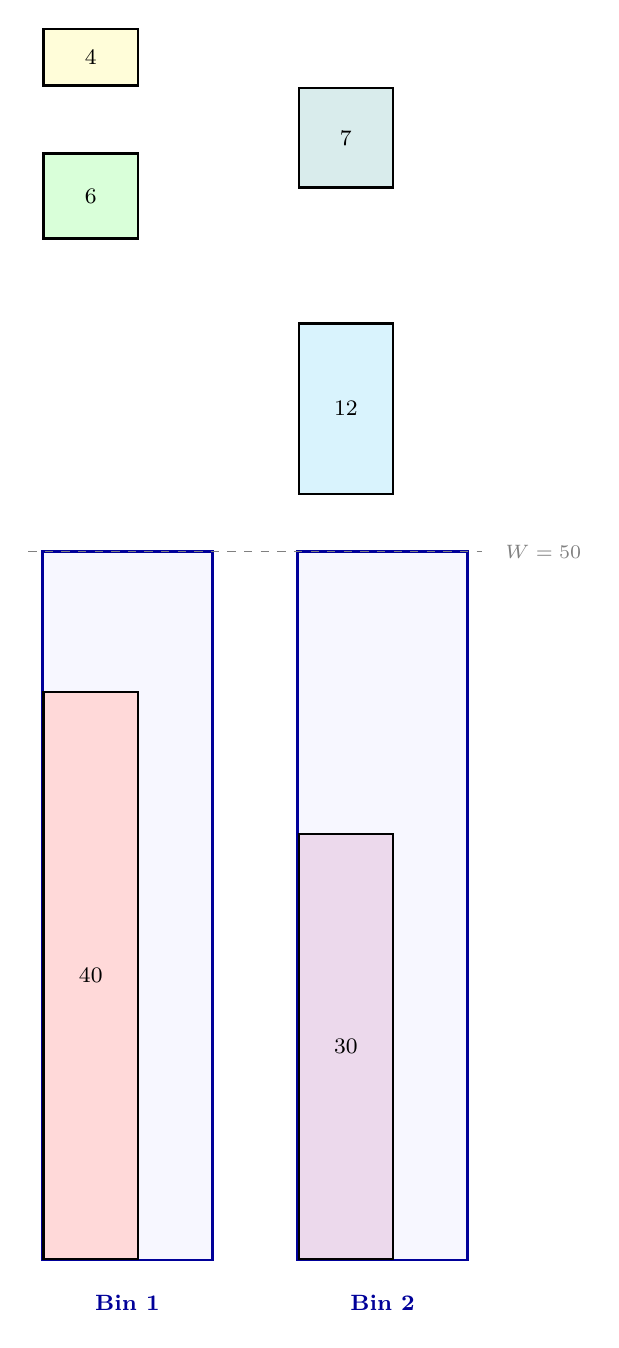
\begin{tikzpicture}[
    x=1.8mm, y=1.8mm,
    bin/.style={draw=blue!60!black, thick, fill=blue!3},
    item/.style={draw, thick, fill=orange!20,
                 font=\footnotesize, anchor=south west},
  ]
  % Bin 1
  \draw[bin] (0,0) rectangle (12, 50);
  \node[font=\footnotesize\bfseries, blue!60!black] at (6, -3) {Bin 1};
  \node[item, fill=red!15,    minimum width=12mm, minimum height=40*1.8mm] at (0, 0) {40};
  \node[item, fill=green!15,  minimum width=12mm, minimum height=6*1.8mm]  at (0, 72) {6};
  \node[item, fill=yellow!15, minimum width=12mm, minimum height=4*1.8mm]  at (0, 82.8) {4};

  % Bin 2
  \draw[bin] (18,0) rectangle (30, 50);
  \node[font=\footnotesize\bfseries, blue!60!black] at (24, -3) {Bin 2};
  \node[item, fill=violet!15, minimum width=12mm, minimum height=30*1.8mm] at (18, 0) {30};
  \node[item, fill=cyan!15,   minimum width=12mm, minimum height=12*1.8mm] at (18, 54) {12};
  \node[item, fill=teal!15,   minimum width=12mm, minimum height=7*1.8mm]  at (18, 75.6) {7};

  % capacity labels
  \draw[gray, dashed] (-1, 50) -- (31, 50);
  \node[font=\scriptsize, gray, anchor=west] at (32, 50) {$W = 50$};
\end{tikzpicture}
\caption{Optimal packing of six items into two bins (capacity 50).
         Bin~1: $40 + 6 + 4 = 50$.  Bin~2: $30 + 12 + 7 = 49$.}
\label{fig:bin-packing-optimal}
\end{figure}
\end{example}

\paragraph{Greedy heuristics for 1D Bin Packing.}

\subparagraph{First Fit (FF).}
Process items in the given order.  Place each item in the
\emph{first} bin where it fits; if none, open a new bin.

\subparagraph{Best Fit (BF).}
Process items in the given order.  Place each item in the bin
that will have the \emph{least remaining capacity} after
insertion (tightest fit); if none, open a new bin.

\subparagraph{First Fit Decreasing (FFD) / Best Fit Decreasing
  (BFD).}
Sort items by \emph{decreasing} size, then apply FF or BF\@.
Sorting large items first is a simple but effective improvement:
large items are the hardest to fit, so placing them early avoids
situations where a large item forces an extra bin at the end.

\begin{example}[Comparing heuristics on \cref{ex:bin-packing-6}]
\label{ex:bin-packing-greedy}
With items in the original order $30, 4, 7, 12, 6, 40$:
\begin{itemize}[nosep]
  \item \textbf{First Fit}: Bin~1 = $\{30, 4, 7, 6\}$ (47),
        Bin~2 = $\{12\}$ (12),
        Bin~3 = $\{40\}$ (40).
        \textbf{3 bins}.
  \item \textbf{Best Fit}: Bin~1 = $\{40, 7\}$ (47),
        Bin~2 = $\{30, 12, 6\}$ (48),
        Bin~3 = $\{4\}$ (4).
        \textbf{3 bins}.
\end{itemize}
With items sorted decreasingly ($40, 30, 12, 7, 6, 4$):
\begin{itemize}[nosep]
  \item \textbf{Best Fit Decreasing}: Bin~1 = $\{40, 7\}$ (47),
        Bin~2 = $\{30, 12, 6, \mathbf{?}\}$---12 + 30 = 42,
        then 6 fits (48), then 4 fits \emph{only in Bin~1}
        (47 + 4 > 50, so new bin).
        Actually: Bin~1 = $\{40, 7\}$, Bin~2 = $\{30, 12, 6\}$,
        Bin~3 = $\{4\}$.  Still \textbf{3 bins}---but on many
        instances BFD significantly outperforms FF\@.
\end{itemize}
The optimum (2 bins) requires a more global view:
Bin~1 = $\{40, 6, 4\}$ (50), Bin~2 = $\{30, 12, 7\}$ (49).
\end{example}

% ------------------------------------------------------------
\subsection{2D and 3D Bin Packing}
\label{ssec:bin-packing-2d3d}
% ------------------------------------------------------------

In higher dimensions, items and bins become geometric objects:

\paragraph{2D Bin Packing.}
Items are \emph{rectangles}; bins are larger rectangles.
Beyond deciding \emph{which} bin, we must decide \emph{where}
in the bin to place each item (coordinates) and possibly whether
to \emph{rotate} it 90\textdegree.

Placement heuristics typically maintain a list of ``corner
points''---positions where a new item can be placed flush against
existing items or bin walls---and choose the corner that wastes
the least space.

\begin{itemize}[nosep]
  \item \textbf{Strip packing}: pack items into horizontal
        strips; each strip is as tall as its tallest item.
        Simple but wastes vertical space.
  \item \textbf{Shelf algorithms}: a refinement of strip
        packing with rules for starting new shelves.
\end{itemize}

\noindent
Applications: cutting glass, wood, or sheet metal; VLSI layout;
page layout.

\begin{remark}[Guillotine cuts]
In glass and wood cutting, every cut must go \emph{edge to edge}
(a ``guillotine cut'').
This rules out L-shaped residual pieces: after cutting, both
resulting pieces must be rectangles.
The constraint significantly restricts the set of feasible
packings and requires specialised algorithms.
\end{remark}

\paragraph{3D Bin Packing / Container Loading.}
Items are \emph{boxes} (rectangular parallelepipeds); bins are
shipping containers.  Additional real-world constraints include:
\begin{itemize}[nosep]
  \item \textbf{Stability}: items must rest on a flat surface;
        no floating items.
  \item \textbf{Fragility}: heavy items cannot be stacked on
        fragile ones.
  \item \textbf{Weight balance}: the centre of gravity must stay
        within tolerance (especially for trucks and aircraft).
  \item \textbf{Rotation restrictions}: some items may only rest
        on certain faces (e.g.\ ``this side up'').
  \item \textbf{Loading order}: items needed first at delivery
        must be accessible (loaded last, near the door).
\end{itemize}

\begin{intermezzo}{From theory to practice}
The gap between textbook bin packing and industrial applications
is large.  A real glass-cutting optimiser must handle guillotine
constraints, material defects, different glass types, and client
grouping (pieces for the same order should come from the same
sheet to simplify logistics).  A container-loading solver must
model gravity, fragility, and access order.  The greedy
heuristics we have seen---First Fit, Best Fit, and their
decreasing variants---serve as building blocks inside these
richer systems, often as the constructive phase of a
metaheuristic.
\end{intermezzo}


% ================================================================
\chapter{C++ Implementation Framework}
% ================================================================
% ============================================================
%  Lecture 5 — C++ recap & software architecture for optimisation
% ============================================================

\section{C++ Recap}
\label{sec:cpp-recap}

From this point on we \emph{implement} the algorithms we study.
The language is C++ (compiled with \texttt{g++} or
\texttt{clang++}).
This section recaps the OOP features we rely on; students
comfortable with all of them can skip ahead to
\cref{sec:solver-architecture}.

% ------------------------------------------------------------
\subsection{Encapsulation and information hiding}
\label{ssec:encapsulation}
% ------------------------------------------------------------

A \textbf{class} bundles \emph{data members} (the state) and
\emph{methods} (the operations on that state) into a single unit.
Access control enforces \emph{information hiding}:

\begin{itemize}[nosep]
  \item \texttt{private} (default for \texttt{class}):
    accessible only within the class itself.
  \item \texttt{protected}: accessible within the class and its
    subclasses.
  \item \texttt{public}: accessible from anywhere.
\end{itemize}

\begin{lstlisting}[language=C++, caption={Basic class layout.}]
class Graph {
public:                     // interface
  Graph(string file_name);  // constructor
  unsigned Nodes() const { return nodes; }
  bool Arc(unsigned i, unsigned j) const;
protected:                  // internal state
  unsigned nodes;
  vector<vector<bool>> adjacency_matrix;
};
\end{lstlisting}

\noindent
The \texttt{const} qualifier on \texttt{Nodes()} promises that
calling it does not modify the object---a crucial contract for
readers of the code and for the compiler's optimiser.

% ------------------------------------------------------------
\subsection{Constructors}
\label{ssec:constructors}
% ------------------------------------------------------------

A \textbf{constructor} initialises an object when it is created.
It has the same name as the class and no return type.
For our optimisation code, the constructor typically reads an
instance from a file:

\begin{lstlisting}[language=C++, caption={Constructor that reads
  from a file.}]
Graph::Graph(string file_name) {
  ifstream is(file_name);
  if (!is) {
    cerr << "Could not open " << file_name << endl;
    exit(1);
  }
  // ... parse the file and fill data members ...
}
\end{lstlisting}

% ------------------------------------------------------------
\subsection{File I/O: \texttt{ifstream} and \texttt{ofstream}}
\label{ssec:file-io}
% ------------------------------------------------------------

The standard library provides \texttt{ifstream} (input) and
\texttt{ofstream} (output) in \texttt{<fstream>}.
They behave like \texttt{cin}/\texttt{cout} but read from / write
to files:

\begin{lstlisting}[language=C++, caption={Reading and writing files.}]
#include <fstream>

ifstream is("instance.txt");   // open for reading
unsigned n;
is >> n;                       // read an integer

ofstream os("solution.txt");   // open for writing
os << "makespan = " << cmax << endl;
\end{lstlisting}

% ------------------------------------------------------------
\subsection{The \texttt{vector} container}
\label{ssec:vector}
% ------------------------------------------------------------

\texttt{std::vector<T>} is a dynamically-sized array.  We use it
everywhere instead of raw C arrays:

\begin{lstlisting}[language=C++, caption={Common \texttt{vector}
  operations.}]
vector<int> v(10, 0);        // 10 elements, all zero
v.push_back(42);             // append
v.size();                    // current length
v[3] = 7;                    // random access (no bounds check)

// 2D: vector of vectors
vector<vector<bool>> matrix(n, vector<bool>(n, false));
\end{lstlisting}

\noindent
For adjacency matrices we use
\texttt{vector<vector<bool>{}>} (compact, random access);
for adjacency lists, \texttt{vector<vector<unsigned>{}>}
(compact, iteration-friendly).


% ============================================================
\section{Software Architecture for Optimisation}
\label{sec:solver-architecture}
% ============================================================

Every solver we build in this course follows the same three-module
architecture:%
\aside{Separating I/O from the solver
lets us swap algorithms without
touching file-parsing code.}

\begin{figure}[H]
\centering
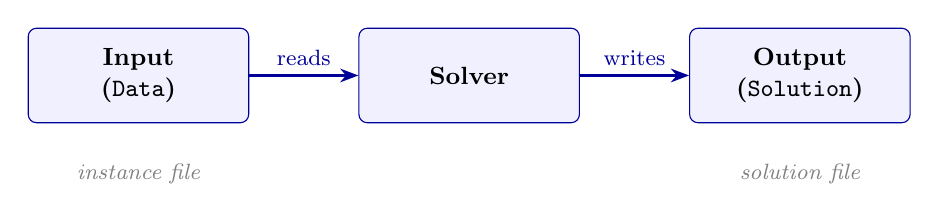
\begin{tikzpicture}[
    box/.style={draw=blue!60!black, fill=blue!6,
                rounded corners=3pt, minimum width=28mm,
                minimum height=12mm, font=\small\bfseries,
                align=center},
    arr/.style={-Stealth, thick, blue!60!black},
    x=42mm, y=16mm
  ]
  \node[box] (inp) at (0, 0) {Input\\(\texttt{Data})};
  \node[box] (sol) at (1, 0) {Solver};
  \node[box] (out) at (2, 0) {Output\\(\texttt{Solution})};

  \draw[arr] (inp) -- (sol) node[midway, above,
    font=\footnotesize] {reads};
  \draw[arr] (sol) -- (out) node[midway, above,
    font=\footnotesize] {writes};

  % file labels
  \node[font=\footnotesize\itshape, text=gray, below=4mm of inp]
    {instance file};
  \node[font=\footnotesize\itshape, text=gray, below=4mm of out]
    {solution file};
\end{tikzpicture}
\caption{Three-module architecture.  The \textbf{Input} class
         reads the instance file and stores the problem data.
         The \textbf{Solver} reads from Input and writes into
         a \textbf{Solution} object.  The Solution class handles
         output formatting.}
\label{fig:three-module}
\end{figure}

\begin{enumerate}
  \item \textbf{Input / Data class.}
    Reads and stores the instance.  Provides read-only accessors
    (\texttt{const} methods) so that the solver cannot
    accidentally modify the input.

  \item \textbf{Output / Solution class.}
    Stores the current solution and provides operators for
    modifying and printing it.

  \item \textbf{Solver.}
    Contains the algorithm logic.  It receives a \texttt{const}
    reference to the Input and produces a Solution.
    Swapping solvers (greedy, backtracking, local search) requires
    no changes to the I/O classes.
\end{enumerate}

This separation is not just good software engineering---it is
essential when comparing multiple algorithms on the same
instances, which is exactly what the course project requires.


% ============================================================
\section{Example: Graph Colouring I/O Classes}
\label{sec:gc-data}
% ============================================================

We illustrate the architecture on the graph colouring problem.
The two files \texttt{GC\_Data.hh} (header) and
\texttt{GC\_Data.cc} (implementation) define the Input and Output
classes.

% ------------------------------------------------------------
\subsection{The \texttt{Graph} class (Input)}
\label{ssec:graph-class}
% ------------------------------------------------------------

\begin{lstlisting}[language=C++,
  caption={\texttt{GC\_Data.hh} --- the \texttt{Graph} class
           (input data).},
  label={lst:gc-data-hh-graph}]
class Graph {
  friend ostream& operator<<(ostream& os, const Graph& g);
public:
  Graph(string file_name);
  unsigned Nodes()   const { return nodes; }
  unsigned Colors()  const { return colors; }
  bool Arc(unsigned i, unsigned j) const
    { return adjacency_matrix[i][j]; }
  unsigned Degree(unsigned i) const
    { return adjacency_list[i].size(); }
  unsigned ArcListMember(unsigned i, unsigned j) const
    { return adjacency_list[i][j]; }
protected:
  unsigned nodes, colors;
  vector<vector<bool>>     adjacency_matrix;
  vector<vector<unsigned>> adjacency_list;
};
\end{lstlisting}

\paragraph{Design notes.}
\begin{itemize}[nosep]
  \item The graph is stored in \emph{two} representations:
    an adjacency matrix (fast $\Oh{1}$ edge queries) and
    adjacency lists (fast neighbour iteration).
    Both are built once by the constructor.
  \item All accessors are \texttt{const}---the solver can read but
    never modify the graph.
  \item The \texttt{friend} declaration lets the \texttt{<\!<}
    operator access private members for printing.
  \item Data members are \texttt{protected} (not \texttt{private})
    so that subclasses---e.g.\ a \texttt{WeightedGraph}---can
    extend them.
\end{itemize}

\paragraph{The constructor} reads a MiniZinc-style data file:

\begin{lstlisting}[language=C++,
  caption={Constructor: reading the instance file.},
  label={lst:gc-constructor}]
Graph::Graph(string file_name) {
  char ch; string buffer; unsigned i, j, val;
  ifstream is(file_name);
  if (!is) { cerr << "Could not open " << file_name << endl; exit(1); }

  is >> buffer >> ch >> nodes  >> ch;  // "nodes = <n>;"
  is >> buffer >> ch >> colors >> ch;  // "colors = <k>;"

  adjacency_matrix.resize(nodes, vector<bool>(nodes, false));
  adjacency_list.resize(nodes);

  is >> buffer >> ch >> ch >> ch;      // "adjacency_matrix = [|"
  for (i = 0; i < nodes; i++)
    for (j = 0; j < nodes; j++) {
      is >> val >> ch;
      if (val == 1 && i < j) {        // upper triangle only
        adjacency_matrix[i][j] = true;
        adjacency_matrix[j][i] = true;
        adjacency_list[i].push_back(j);
        adjacency_list[j].push_back(i);
      }
    }
}
\end{lstlisting}

\noindent
The file format matches MiniZinc's data syntax (which we will
use in the next lectures), so the same instance file serves both
the C++ solver and the MiniZinc model.

% ------------------------------------------------------------
\subsection{The \texttt{Coloring} class (Output)}
\label{ssec:coloring-class}
% ------------------------------------------------------------

\begin{lstlisting}[language=C++,
  caption={\texttt{GC\_Data.hh} --- the \texttt{Coloring} class
           (solution).},
  label={lst:gc-data-hh-coloring}]
class Coloring {
  friend ostream& operator<<(ostream& os, const Coloring& col);
public:
  Coloring(const Graph& my_in)
    : in(my_in), coloring(in.Nodes(), -1) {}
  void Reset();
  int  operator[](unsigned i) const { return coloring[i]; }
  int& operator[](unsigned i)       { return coloring[i]; }
protected:
  const Graph& in;
  vector<int>  coloring;
};
\end{lstlisting}

\paragraph{Design notes.}
\begin{itemize}[nosep]
  \item The constructor takes a \texttt{const Graph\&} and
    initialises every node's colour to $-1$ (uncoloured).
  \item The \texttt{operator[]} overloads provide array-like
    syntax: \texttt{col[v] = 3} assigns colour~3 to node~$v$;
    \texttt{col[v]} reads it.
    The \texttt{const} version returns by value (read-only);
    the non-\texttt{const} version returns by reference
    (read-write).
  \item \texttt{Reset()} sets all colours back to $-1$, allowing
    the solver to restart without reallocating memory.
  \item The \texttt{in} reference lets the output class access
    graph data (e.g.\ number of nodes) without duplicating it.
\end{itemize}

\begin{observation}
This pattern---\texttt{Data} class with \texttt{const} accessors,
\texttt{Solution} class with a reference to the data---recurs in
every problem we implement.  For TSP: \texttt{TSP\_Data} stores
the distance matrix, \texttt{TSP\_Solution} stores the tour.
For bin packing: \texttt{BP\_Data} stores item sizes and bin
capacity, \texttt{BP\_Solution} stores the assignment of items to
bins.  The solver is always a separate function or class that
reads from \texttt{Data} and writes to \texttt{Solution}.
\end{observation}


% ============================================================
\section{Implementing Greedy: DSatur for Graph Colouring}
\label{sec:gc-greedy-impl}
% ============================================================

With the architecture in place, let us implement the DSatur
algorithm from \cref{ssec:dsatur}.
The solver lives in its own compilation unit
(\texttt{GC\_Greedy.hh/cc}), separate from the I/O classes.

% ------------------------------------------------------------
\subsection{The solver loop}
\label{ssec:gc-greedy-loop}
% ------------------------------------------------------------

\begin{lstlisting}[language=C++,
  caption={DSatur main loop (\texttt{GC\_Greedy.cc}).},
  label={lst:gc-greedy-loop}]
void GreedyGCSolver(const Graph& in, Coloring& out) {
  unsigned i, k, c;
  int n;
  // colors[v] = set of colours still available for vertex v
  vector<vector<unsigned>> colors(
      in.Nodes(), vector<unsigned>(in.Colors()));
  for (i = 0; i < in.Nodes(); i++)
    iota(colors[i].begin(), colors[i].end(), 0);

  out.Reset();
  for (i = 0; i < in.Nodes(); i++) {
    n = SelectNode(colors, in, out);  // DSatur selection
    if (colors[n].size() == 0)
      return;  // no feasible colour: search fails
    k = Random(0, colors[n].size() - 1);
    c = colors[n][k];                 // random among available
    Update(n, c, colors, in);         // propagate
    out[n] = c;
  }
}
\end{lstlisting}

\paragraph{Key data structure.}
\texttt{colors[v]} is the list of colours still available for
vertex~$v$.  Initially every vertex has all $k$ colours.
After colouring a vertex, \texttt{Update} removes that colour
from every neighbour's list.
The \emph{saturation degree} of $v$ is implicitly
$k - |\texttt{colors[v]}|$: fewer available colours $=$ higher
saturation.

% ------------------------------------------------------------
\subsection{Node selection (DSatur rule)}
\label{ssec:gc-select-node}
% ------------------------------------------------------------

\begin{lstlisting}[language=C++,
  caption={\texttt{SelectNode}: pick the most saturated
           uncoloured vertex.},
  label={lst:gc-select}]
unsigned SelectNode(const vector<vector<unsigned>>& v,
                    const Graph& in, const Coloring& out) {
  unsigned i;
  int best = -1;
  for (i = 0; i < v.size(); i++)
    if (out[i] == -1 &&               // uncoloured
        (best == -1
         || v[i].size() < v[best].size()    // fewer available
         || (v[i].size() == v[best].size()
             && in.Degree(i) > in.Degree(best))))
      best = i;                        // tie-break: degree
  return best;
}
\end{lstlisting}

\noindent
Smaller \texttt{colors[v].size()} means higher saturation.
Ties broken by highest degree---exactly the DSatur rule.

% ------------------------------------------------------------
\subsection{Propagation}
\label{ssec:gc-update}
% ------------------------------------------------------------

\begin{lstlisting}[language=C++,
  caption={\texttt{Update}: remove colour \texttt{c} from
           all neighbours of~\texttt{n}.},
  label={lst:gc-update}]
void Update(unsigned n, unsigned c,
            vector<vector<unsigned>>& v, const Graph& in) {
  for (unsigned i = 0; i < in.Degree(n); i++) {
    unsigned k = in.ArcListMember(n, i);
    for (unsigned j = 0; j < v[k].size(); j++)
      if (v[k][j] == c) {
        v[k].erase(v[k].begin() + j);
        break;
      }
  }
}
\end{lstlisting}

% ------------------------------------------------------------
\subsection{Driver and Makefile}
\label{ssec:gc-driver}
% ------------------------------------------------------------

\begin{lstlisting}[language=C++,
  caption={Minimal driver (\texttt{GC\_Driver.cc}).},
  label={lst:gc-driver}]
#include "GC_Data.hh"
#include "GC_Greedy.hh"

int main(int argc, char* argv[]) {
  if (argc != 2) {
    cerr << "Usage: " << argv[0] << " <input_file>" << endl;
    return 1;
  }
  Graph in(argv[1]);
  Coloring out(in);
  GreedyGCSolver(in, out);
  cout << out << endl;
  return 0;
}
\end{lstlisting}

\noindent
The driver is trivially short: create Input, create Output, run
Solver, print.  To switch algorithms, only the solver call
changes.

\begin{lstlisting}[language=make,
  caption={Makefile for the graph colouring solver.},
  label={lst:gc-makefile}]
OPTIONS = -Wall -Wfatal-errors -O3

GC_Test.exe: GC_Driver.o GC_Greedy.o GC_Data.o Random.o
    g++ -o GC_Test.exe $^

GC_Data.o: GC_Data.cc GC_Data.hh
    g++ $(OPTIONS) -c GC_Data.cc

GC_Greedy.o: GC_Greedy.cc GC_Greedy.hh GC_Data.hh
    g++ $(OPTIONS) -c GC_Greedy.cc

GC_Driver.o: GC_Driver.cc GC_Data.hh
    g++ $(OPTIONS) -c GC_Driver.cc

clean:
    rm -f *.o GC_Test.exe
\end{lstlisting}


% ============================================================
\section{Example 2: Bus Driver Scheduling (I/O classes)}
\label{sec:bds-data}
% ============================================================

As a second example of the Input/Output pattern, we look at the
\textbf{Bus Driver Scheduling} (BDS) problem: given a set of
\emph{tasks} (bus trips) and a set of \emph{shifts} (driver
work-blocks, each covering certain tasks), select a minimum-cost
set of shifts that covers every task.%
\aside{BDS is a set-covering problem:
shifts = sets, tasks = elements.}

\begin{lstlisting}[language=C++,
  caption={\texttt{BDS\_Data.hh} --- Input class (excerpt).},
  label={lst:bds-input}]
class BDS_Input {
  friend ostream& operator<<(ostream& os, const BDS_Input& bs);
public:
  BDS_Input(string file_name);
  unsigned Tasks()  const { return tasks; }
  unsigned Shifts() const { return shifts; }
  bool Covers(unsigned s, unsigned t) const
    { return covers[s][t]; }
  unsigned ShiftCost(unsigned s) const
    { return shift_cost[s]; }
protected:
  unsigned tasks, shifts;
  vector<unsigned> shift_cost;
  vector<vector<bool>> covers;
  vector<vector<unsigned>> shift_members;
  vector<vector<unsigned>> task_coverage;
};
\end{lstlisting}

\begin{lstlisting}[language=C++,
  caption={\texttt{BDS\_Data.hh} --- Output class (excerpt).},
  label={lst:bds-output}]
class BDS_Output {
  friend ostream& operator<<(ostream& os, const BDS_Output& out);
public:
  BDS_Output(const BDS_Input& i);
  bool operator[](unsigned s) const
    { return selected_shifts[s]; }
  unsigned Uncovered() const { return uncovered; }
  unsigned TotalCost() const { return total_cost; }

  void InsertShift(unsigned s);
  void RemoveShift(unsigned s);
  void RemoveAll();
private:
  const BDS_Input& in;
  vector<bool> selected_shifts;
  vector<unsigned> coverage;
  unsigned uncovered, total_cost;
};
\end{lstlisting}

\paragraph{Design notes.}
\begin{itemize}[nosep]
  \item The Output class maintains \emph{incremental}
    bookkeeping: \texttt{InsertShift} and \texttt{RemoveShift}
    update \texttt{coverage}, \texttt{uncovered}, and
    \texttt{total\_cost} without a full recount.
  \item This incremental pattern will be essential for
    \emph{local search} (later chapters), where we repeatedly
    insert/remove shifts and need fast cost evaluation.
  \item The same Input/Output split applies: greedy,
    backtracking, or local-search solvers all use the same
    \texttt{BDS\_Input} and \texttt{BDS\_Output}.
\end{itemize}


% ================================================================
\chapter{Single-Machine Scheduling}
% ================================================================
% \input{chapters/03-single-machine}

% ================================================================
\chapter{Parallel-Machine Scheduling}
% ================================================================
% \input{chapters/03-parallel-machine}

% ================================================================
\chapter{Flow Shop \& Job Shop Scheduling}
% ================================================================
% \input{chapters/04-flow-job-shop}

% ================================================================
\chapter{Metaheuristics for Scheduling}
% ================================================================
% \input{chapters/05-metaheuristics}

\end{document}
